
\subsection{Considerações Iniciais}

\begin{frame}{Considerações Iniciais}

No dimensionamento de um projeto de SFV se faz necessário responder as duas questões a seguir:

\vspace{.5cm}

\begin{enumerate}
\item Quantidade de energia disponível no local?
\item Quantidade de energia consumida pela carga?
\end{enumerate}

\vspace{.5cm}

\begin{exampleblock}{}
\begin{center}
Respondidas as duas questões um SFV pode ser projetado, seja ele conectado à rede ou não
\end{center} 
\end{exampleblock}

\end{frame}

%----------------------->
\subsection{Quantidade de energia consumida pela carga}
%----------------------->

\begin{frame}{Energia consumida pela carga}

Quanta é a \textbf{energia consumida} diariamente no local ? 

\begin{figure}[H]
	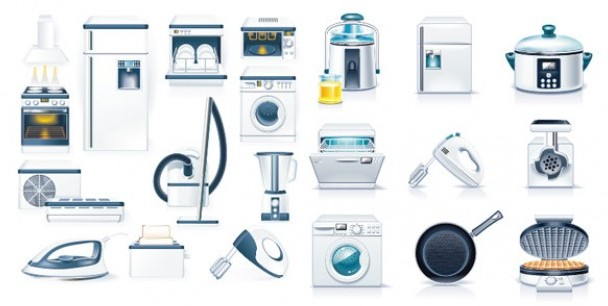
\includegraphics[scale=.7,center]{eletrodomesticos}
\end{figure}

\end{frame}

\begin{frame}{Energia consumida pela carga}

Para calcular o consumo de um determinado local, se faz necessário fazer a lista dos itens que consumem energia 

\vspace{.5cm}

\begin{columns}[T]
    \begin{column}{0.5\textwidth}
		\begin{alertblock}{Potência do equipamento}
			\begin{itemize}
			\item Placa de identificação
			\item Catalogo do fabricante
			\end{itemize}
		\end{alertblock}
    \end{column}
    \begin{column}{0.5\textwidth}  
    	\begin{alertblock}{Tempo de uso}
			\begin{itemize}
			\item Horas por dia
			\item Hábitos de consumo	
			\end{itemize}
		\end{alertblock}  		
    \end{column}
\end{columns}

\vspace{.5cm}

\begin{center}
\begin{equation*}
\underset{Consumida}{Energia}\left [ kWh \right ]=\sum \underset{do \; Equipamento}{Pot\hat{e}ncia}\left [ kW \right ] \times \underset{de \; Uso}{Tempo}\left [ h \right ]
\end{equation*}
\end{center} 

\end{frame}

\begin{frame}{Energia consumida pela carga}

\begin{figure}[H]
	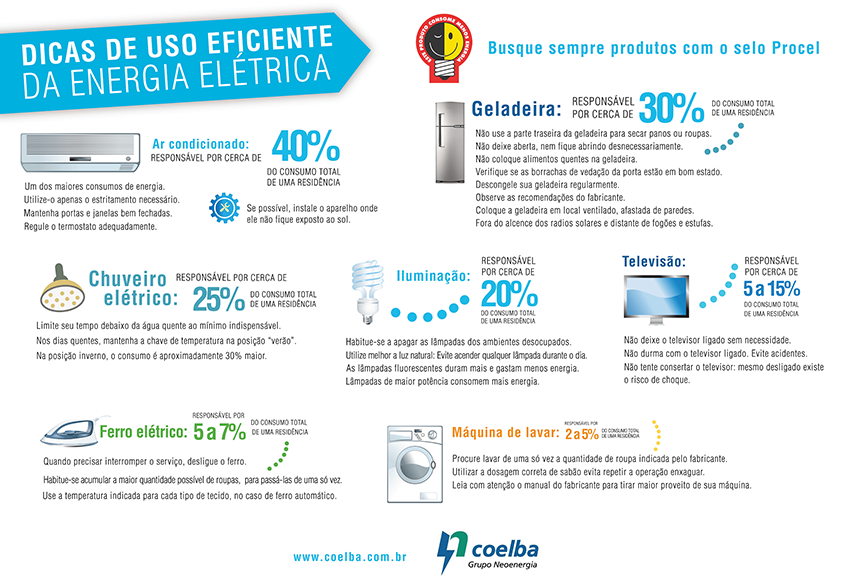
\includegraphics[scale=.5,center]{infografico-coelba}
\end{figure}

\end{frame}

\begin{frame}{Energia consumida pela carga}

\begin{columns}[T]
    \begin{column}{0.5\textwidth}
		\vspace{1cm}
		Quais são seus hábitos de consumo de energia elétrica?
	    \vspace{.5cm}
    	\begin{figure}[H]
			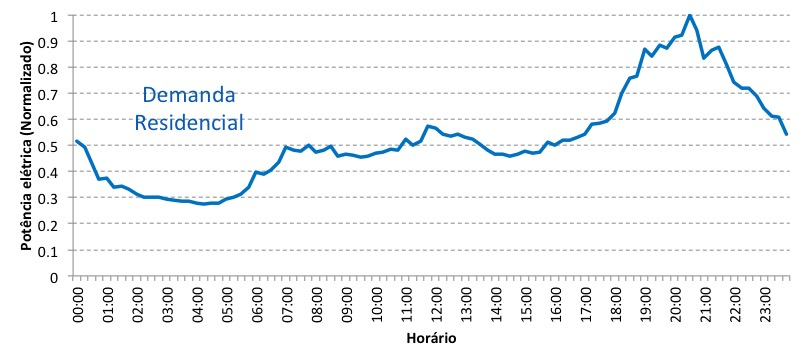
\includegraphics[scale=.2,left]{curva_residencial}
		\end{figure}
    \end{column}
    \begin{column}{0.5\textwidth} 
		\begin{figure}[H]
			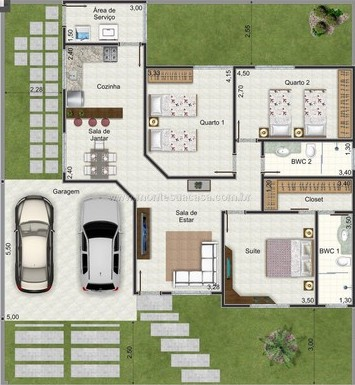
\includegraphics[scale=.45,right]{planta_casa}
		\end{figure}  		
    \end{column}
\end{columns}


\end{frame}

\begin{frame}{Energia consumida pela carga}

Em instalações Off-Grid, a energia consumida pode ser estimada a partir do cálculo do consumo médio, máximo ou mínimo sazonal de eletrodomésticos de acordo com um uso hipotético. 

\begin{equation*}
\underset{M\acute{e}dia \, Mensal}{Consumo}\left [ kWh \right ]=\underset{Equipamento}{Pot\hat{e}ncia}\left [ W \right ]\times\underset{M\acute{e}dia \, Diaria}{Uso}\left [ \frac{h}{dia} \right ]\times\underset{M\hat{e}s}{Uso}\left [  \frac{dia}{M\hat{e}s} \right ]
\end{equation*}

\begin{figure}[H]
	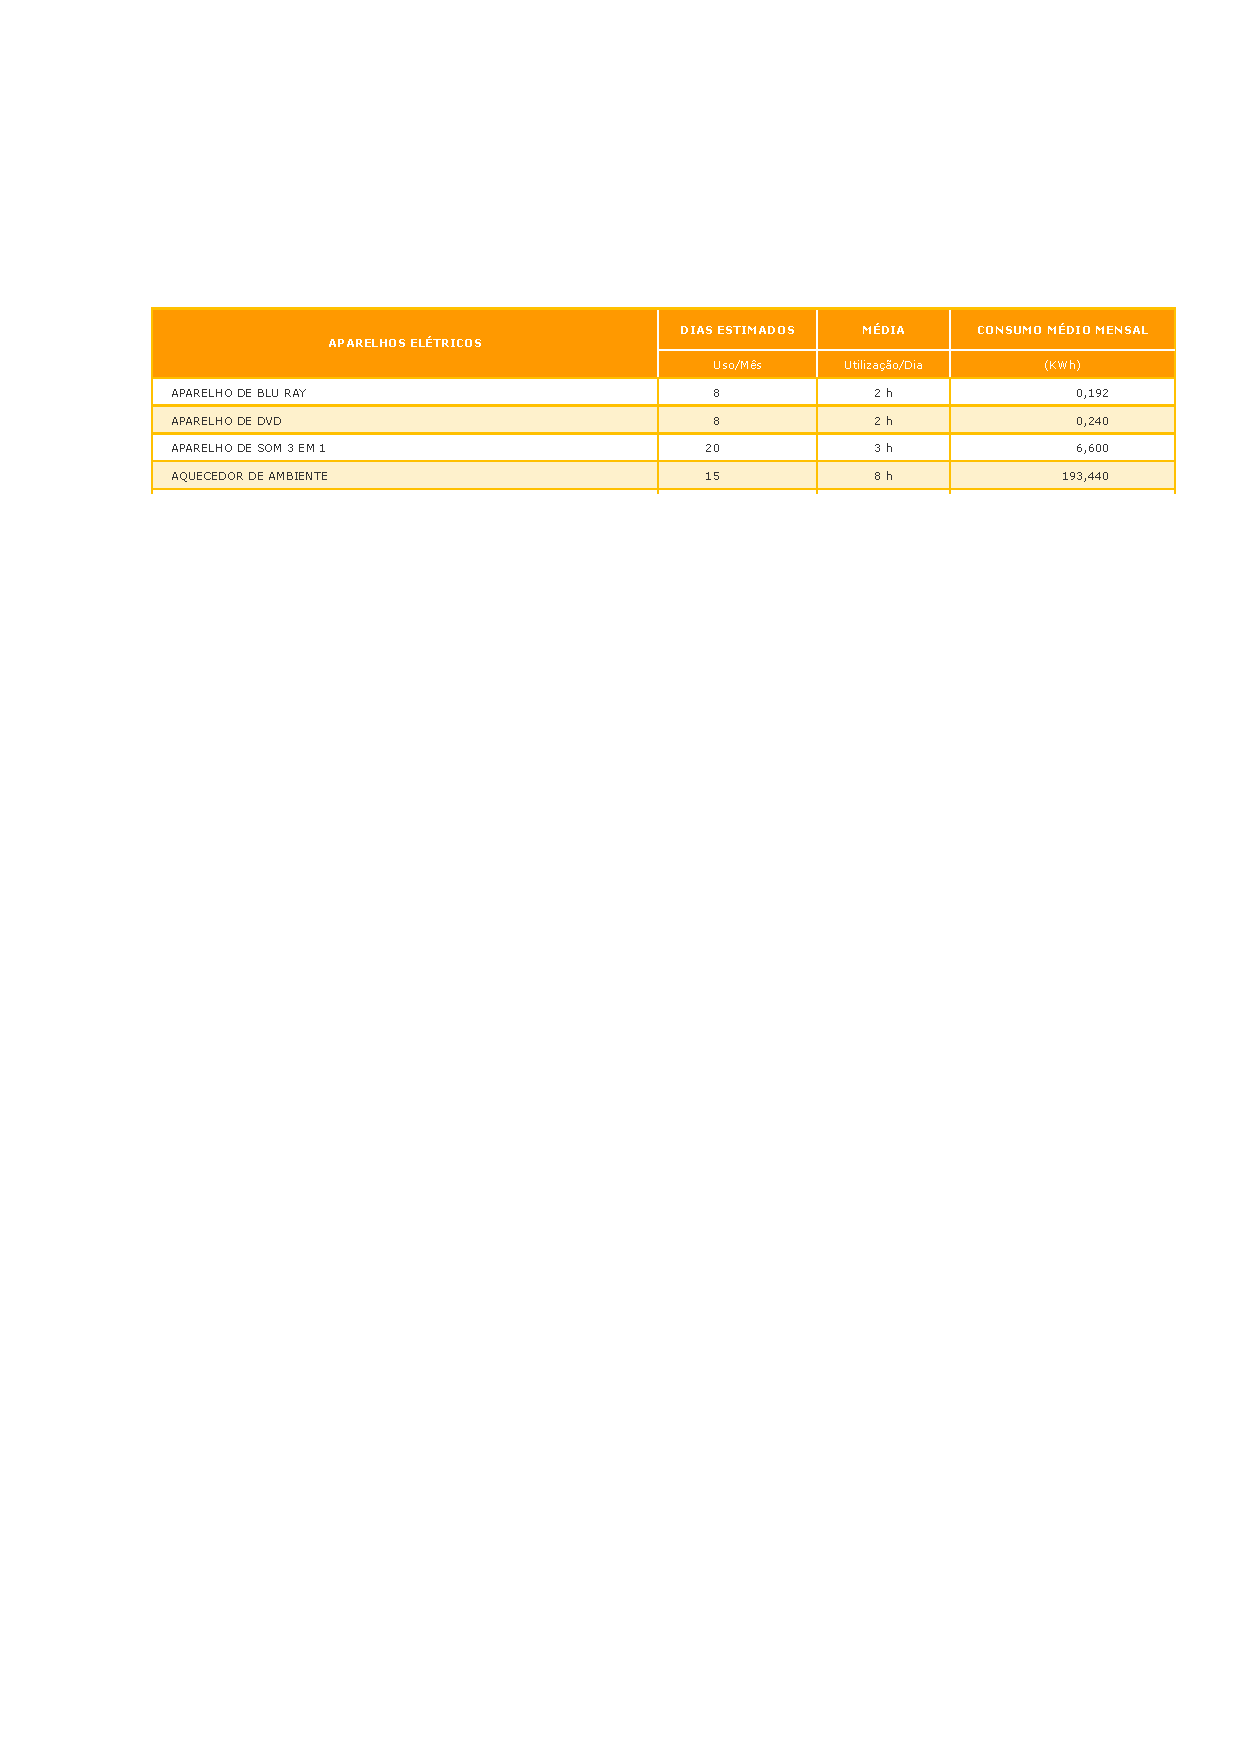
\includegraphics[scale=.6,center]{Tabela-Consumo-Equipamentos-Procel-Eletrobras}
\end{figure}

%\begin{equation*}
%\underset{Mensal}{Custo}\left [ R\$ \right ]=\underset{M\acute{e}dia \, Mensal}{Consumo}\left [ kWh \right ]\times\underset{Concession\acute{a}ria}{Tarifa}\left [ \frac{R\$}{kWh} \right ]
%\end{equation*}

%\begin{exampleblock}{}
%\begin{center}
%A identificação de cargas consideradas como críticas, pode ajudar no dimensionamento de um sistema de armazenamento com baterias
%\end{center} 
%\end{exampleblock}

\end{frame}

\begin{frame}{Energia consumida pela carga}

Em instalações On-Grid, a energia consumida pode ser estimada usando os últimos 12 meses das faturas de eletricidade existentes

\begin{figure}[H]
	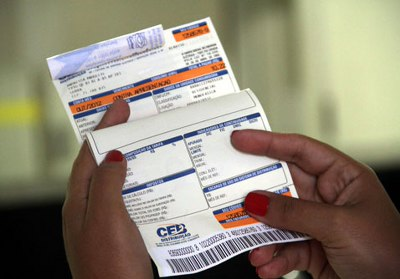
\includegraphics[scale=.5,center]{conta_ceb}
\end{figure}

\end{frame}

%----------------------->
\subsection{Quantidade de energia disponível no local}
%----------------------->

\begin{frame}{Energia disponível no local}

Quanta é a \textbf{energia produzida} diariamente pelos módulos fotovoltaicos? 

\begin{figure}[H]
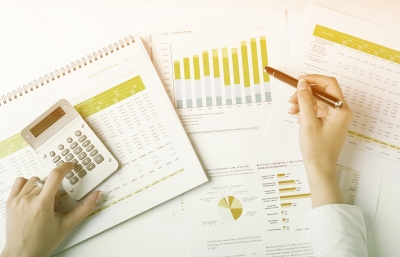
\includegraphics[scale=.7,center]{09}
\end{figure}

\end{frame}

\begin{frame}{Energia disponível no local}

Os movimentos da Terra, combinados com as questões ambientais, são fatores que influenciam a quantidade de radiação solar do local

\vspace{.5cm}

\begin{columns}[T]
    \begin{column}{0.5\textwidth}
		\centering
		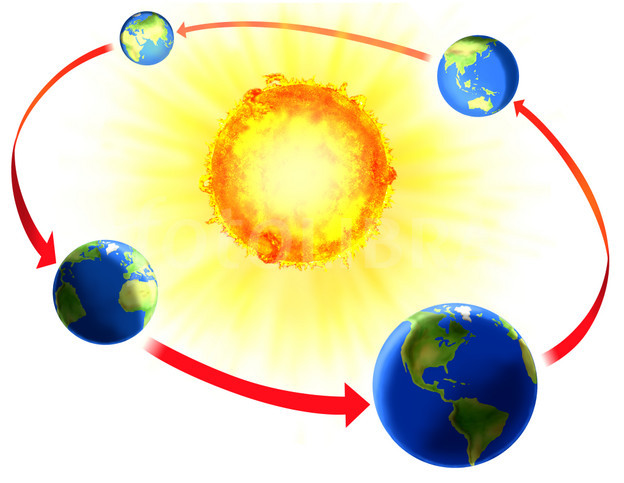
\includegraphics[scale=.2,center]{rota_trans}
    \end{column}
    \begin{column}{0.5\textwidth}    
		\centering
      	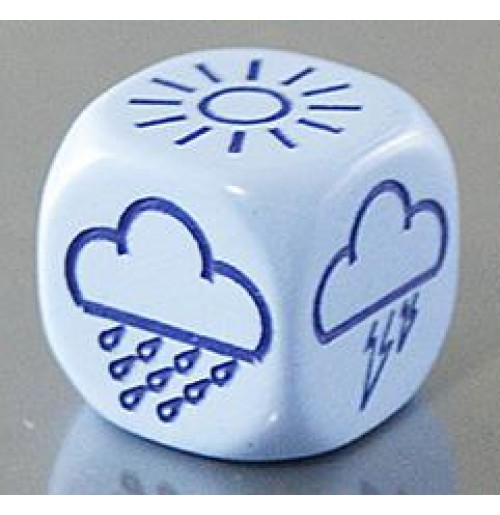
\includegraphics[scale=.2,center]{clima}
    \end{column}
\end{columns}

\end{frame}

\begin{frame}{Energia disponível no local}

A cálculo da energia disponível são necessárias as informações a seguir:

\vspace{.5cm}

\begin{columns}[T]
    \begin{column}{0.5\textwidth}
		Mapas solarimétricos
		\begin{itemize}
			\item Condições de irradiação diária
			\item Quantidade de horas diárias de Sol pleno
		\end{itemize}
		\vspace{.5cm}
		Catálogos dos fabricantes
		\begin{itemize}
			\item Especificações do módulo
		\end{itemize}
    \end{column}
    \begin{column}{0.5\textwidth}    
		\centering
      	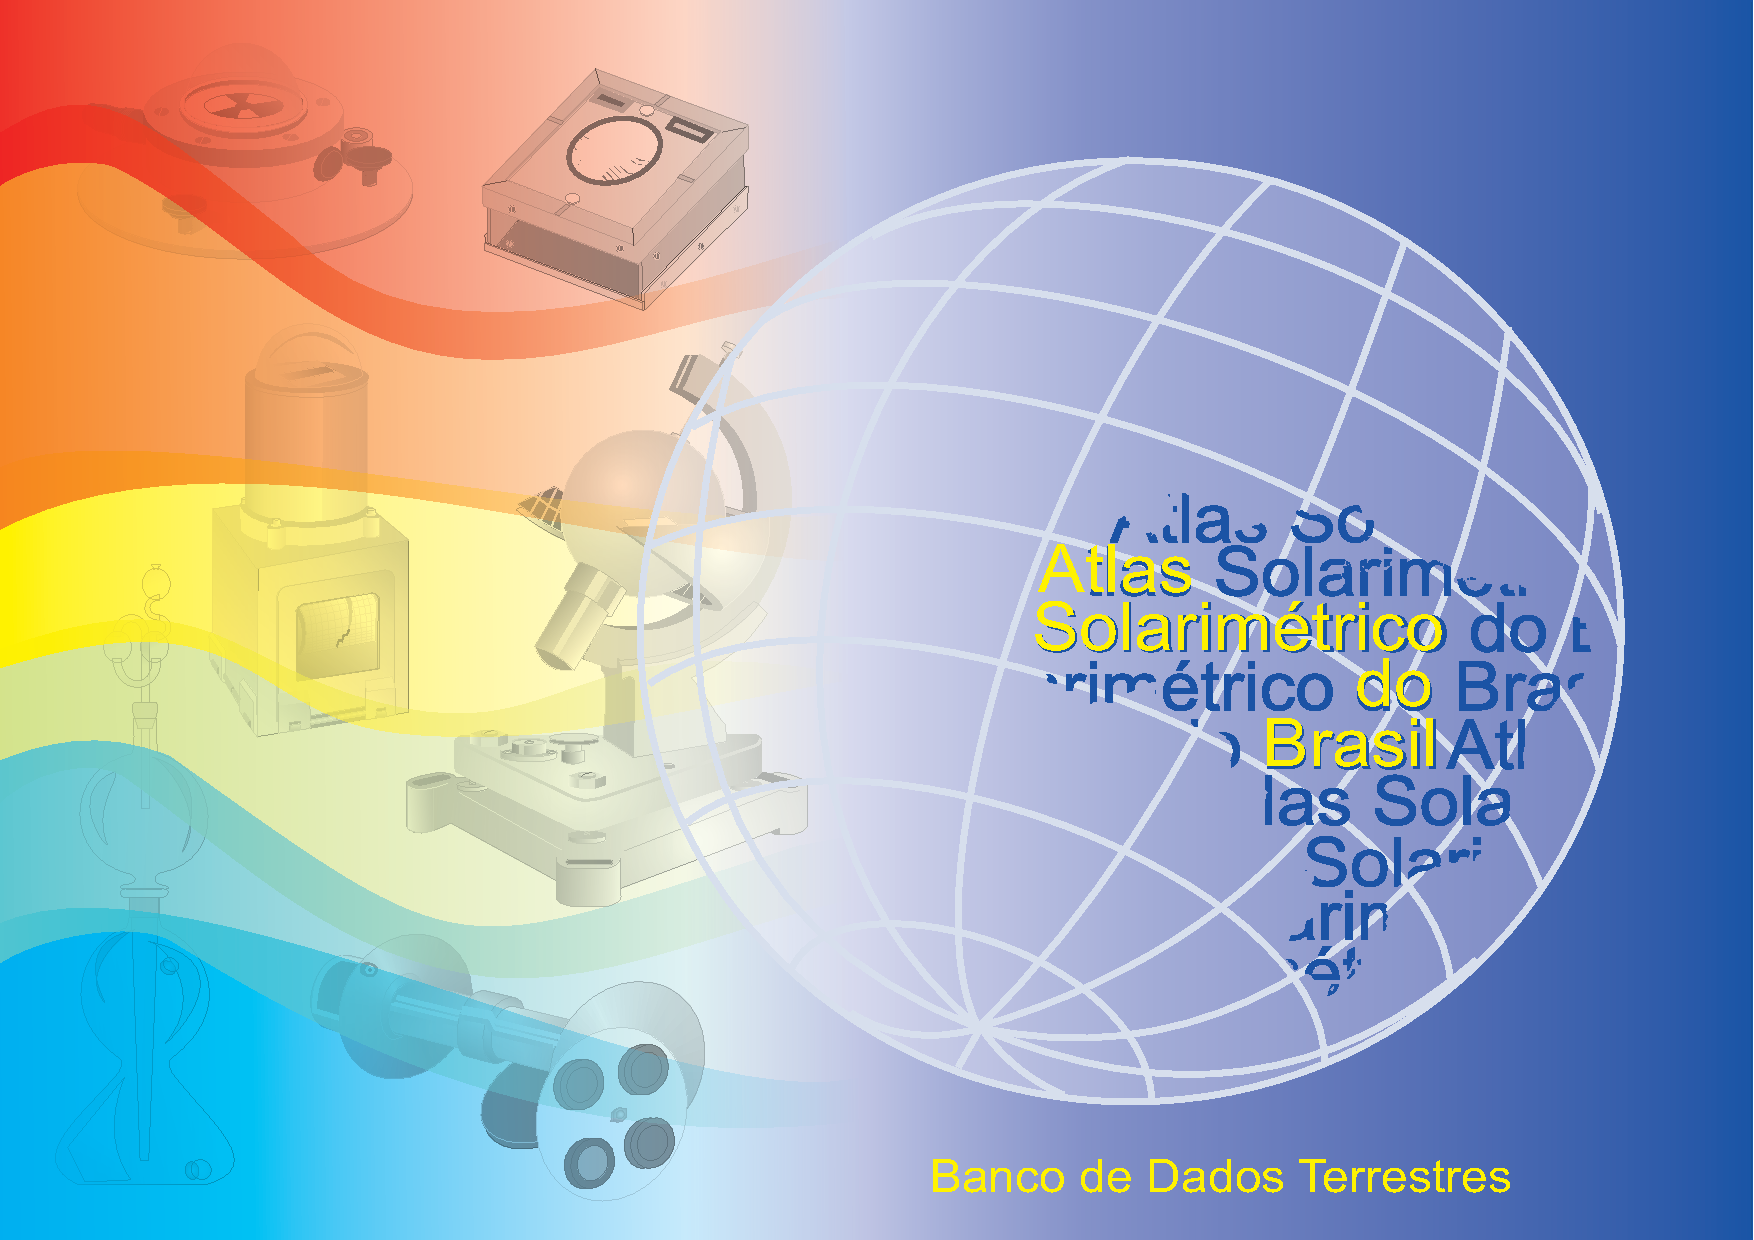
\includegraphics[scale=.2,center]{atlas}
    \end{column}
\end{columns}

\end{frame}

\begin{frame}{Energia disponível no local}

\begin{columns}[T]
    \begin{column}{0.5\textwidth}
    	\centering
      	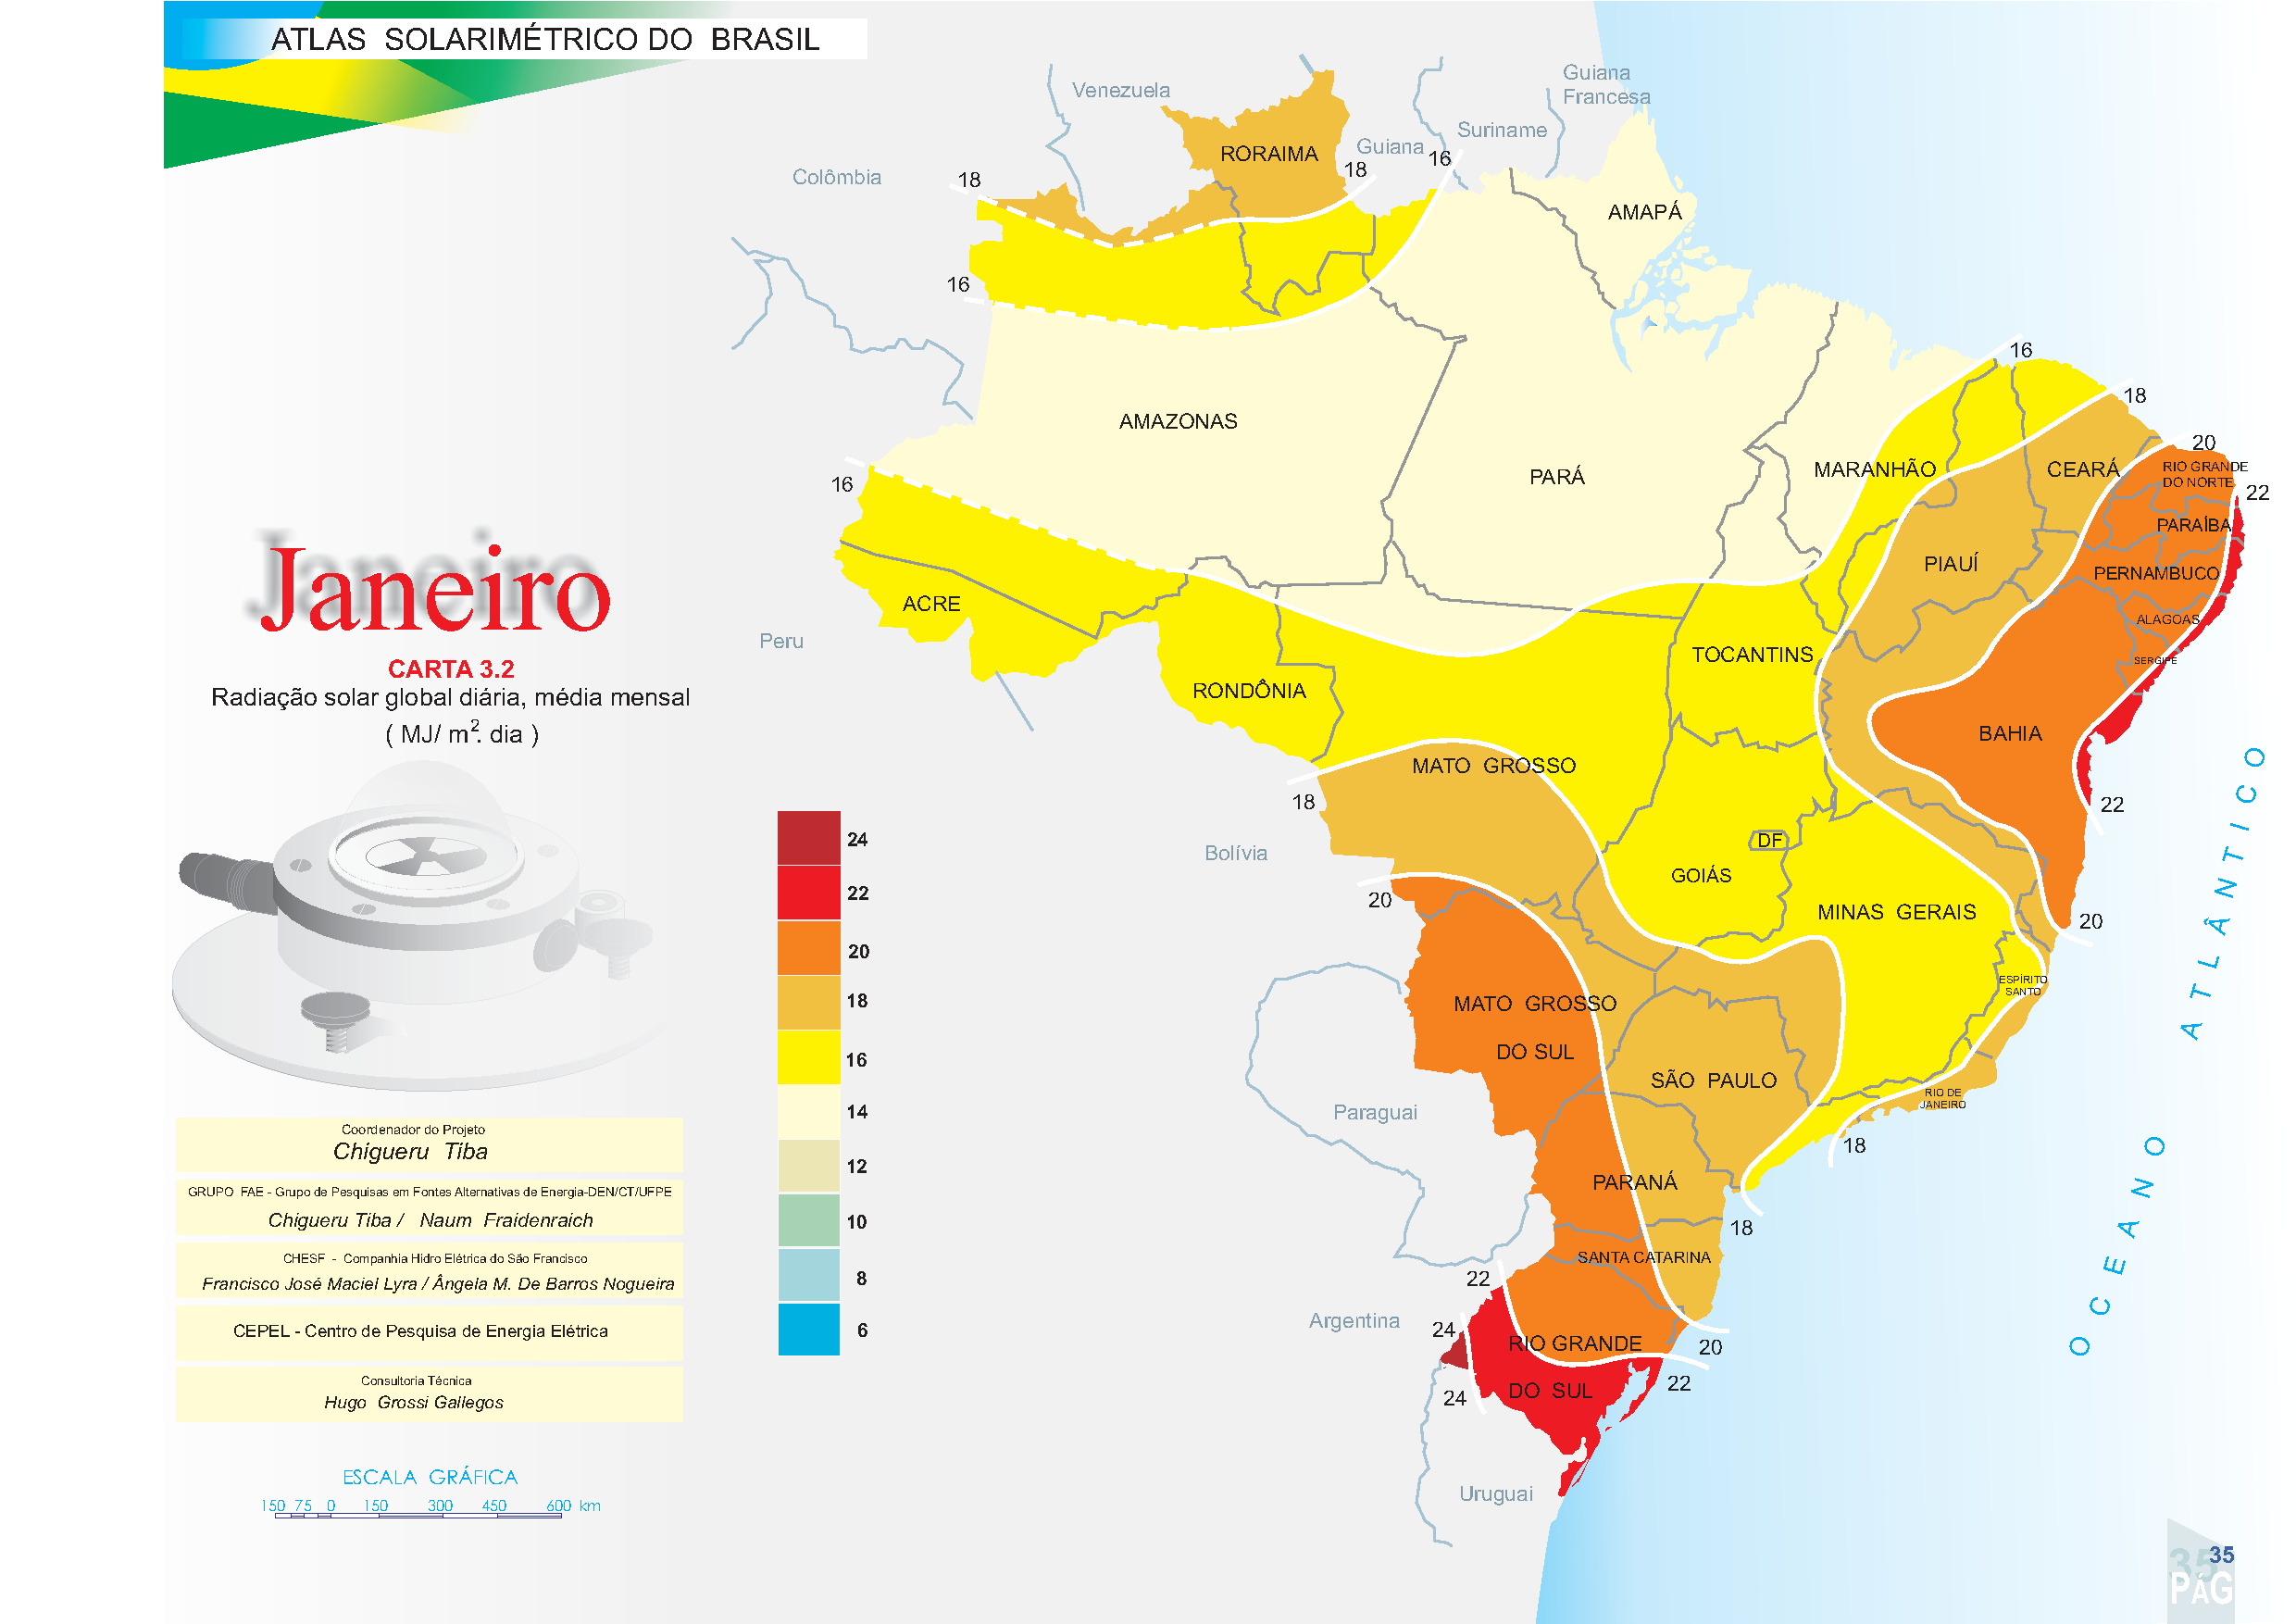
\includegraphics[scale=.12,center]{atlas_irra_jan}
    \end{column}
    \begin{column}{0.5\textwidth}
    	\centering
      	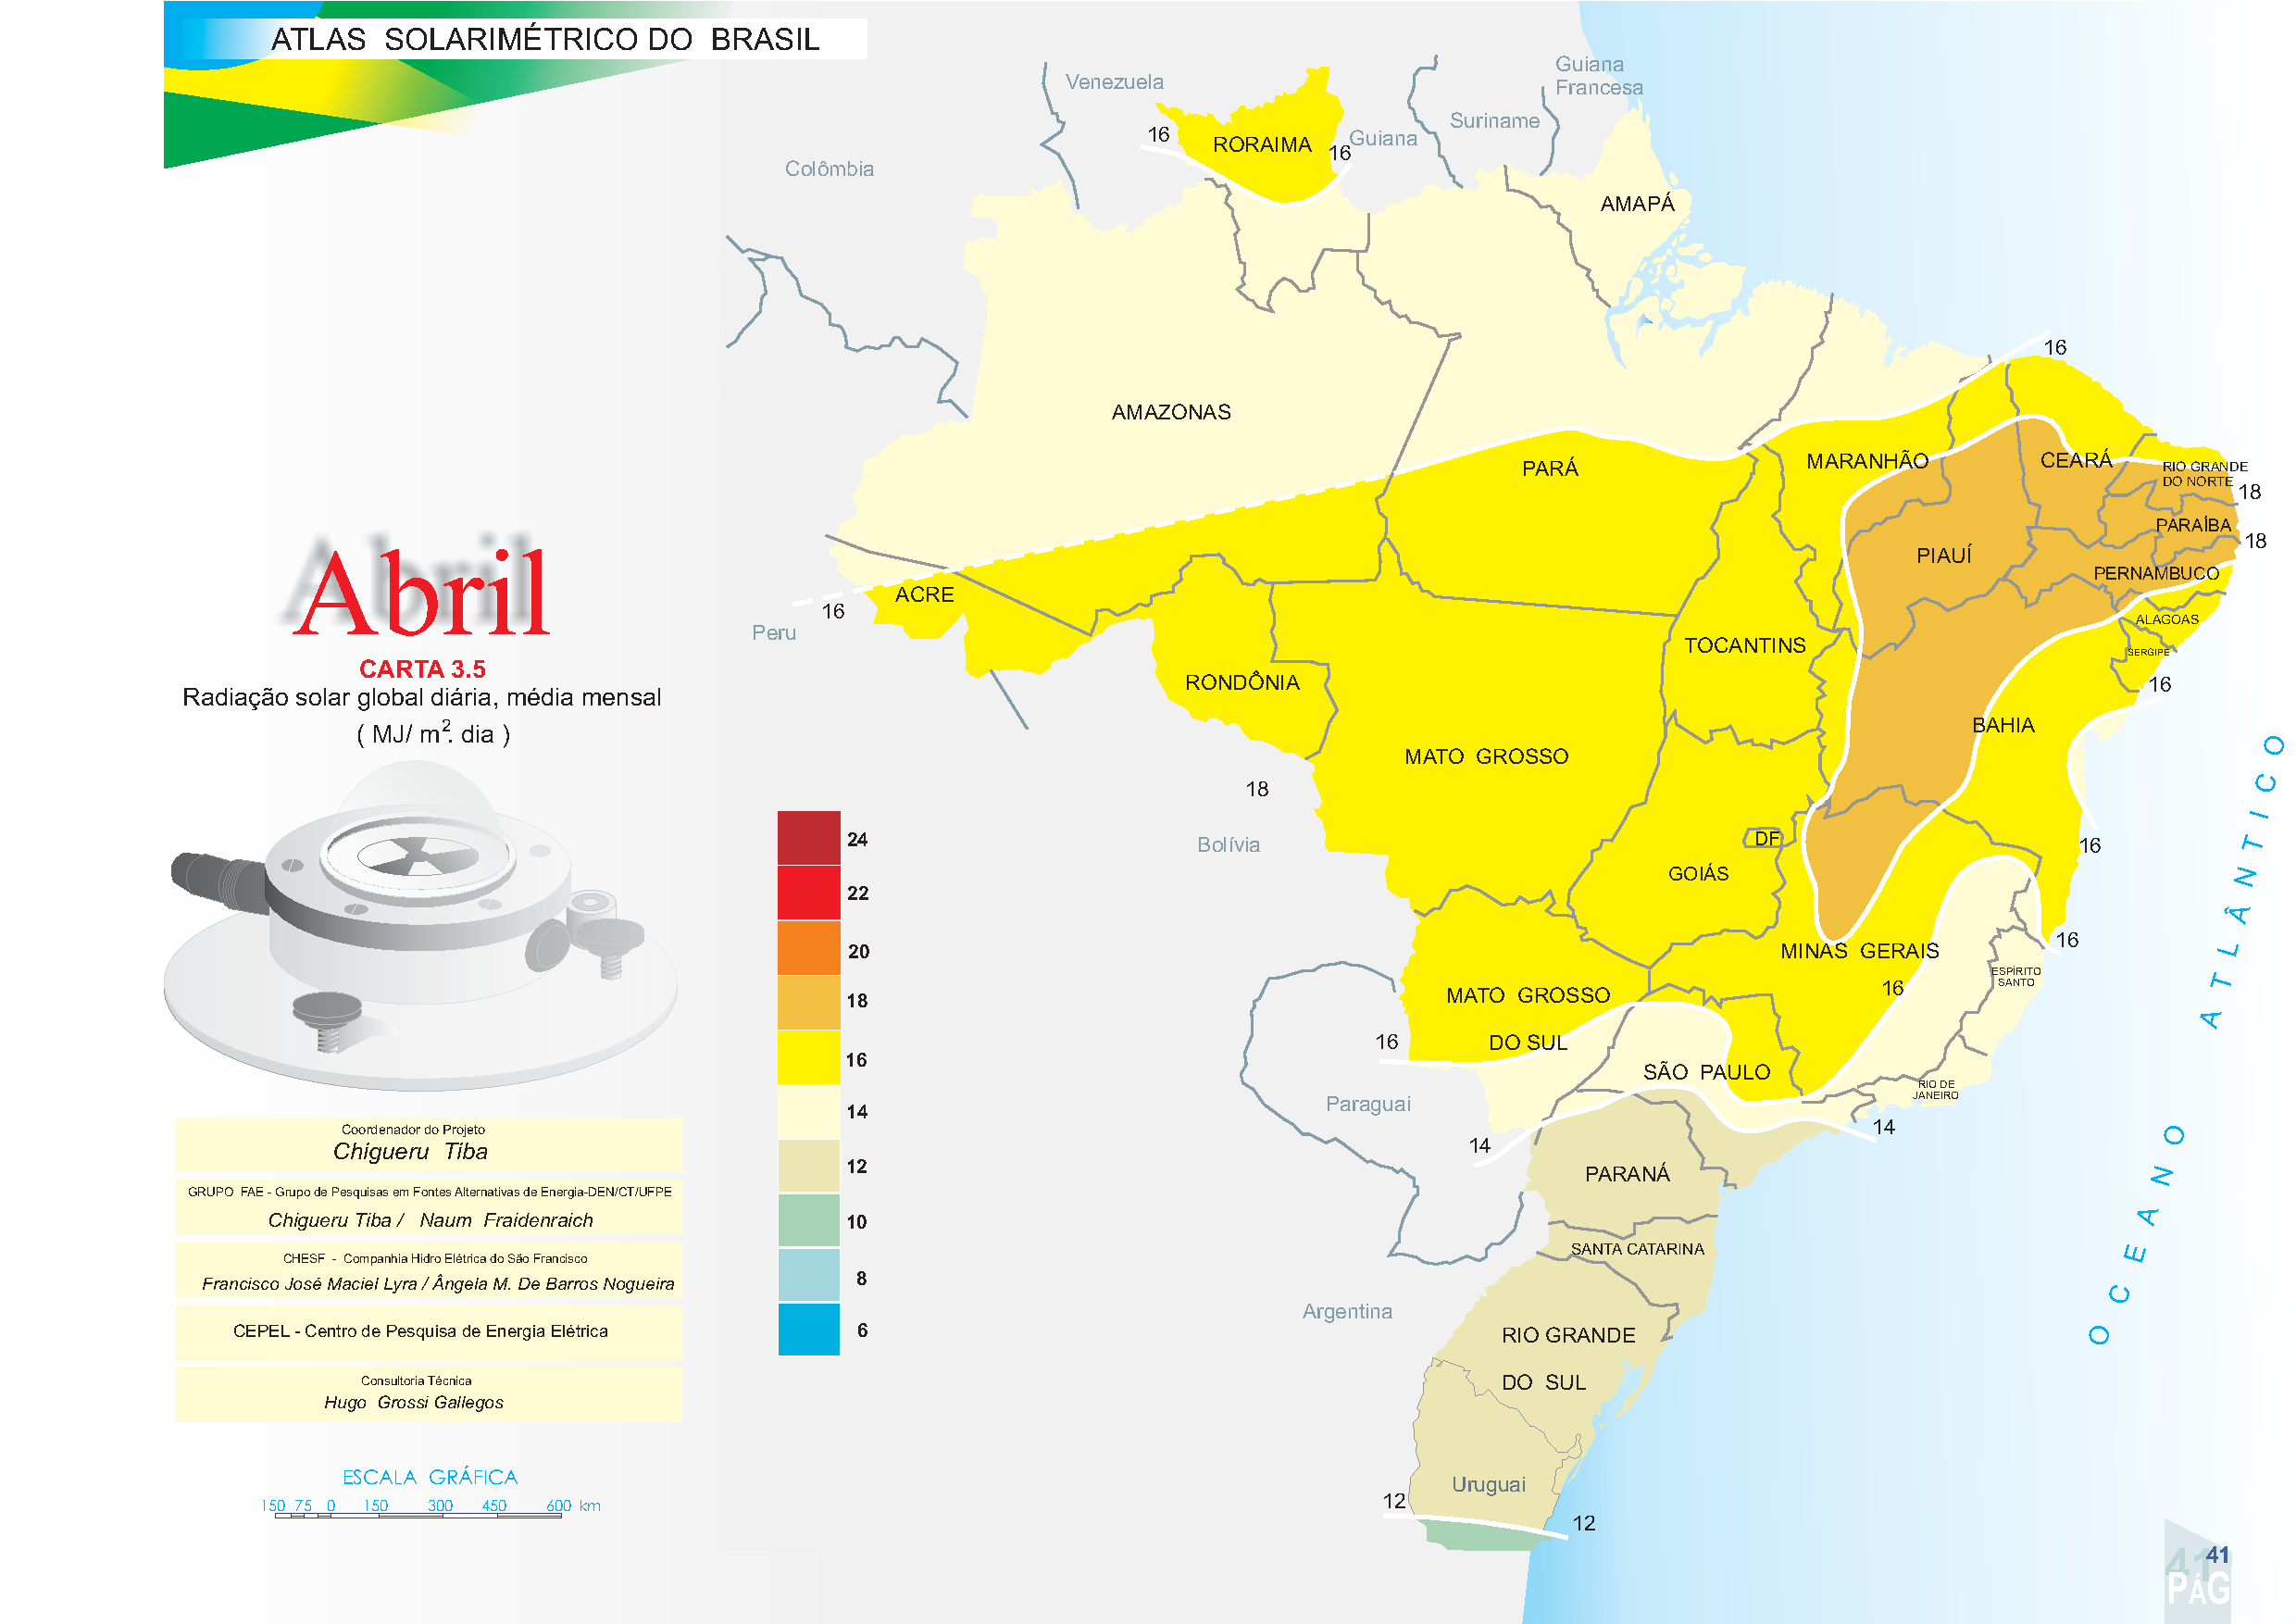
\includegraphics[scale=.12,center]{atlas_irra_abr}
    \end{column}
\end{columns}

\vspace{.25cm}

\begin{columns}[T]
    \begin{column}{0.5\textwidth}
    	\centering
      	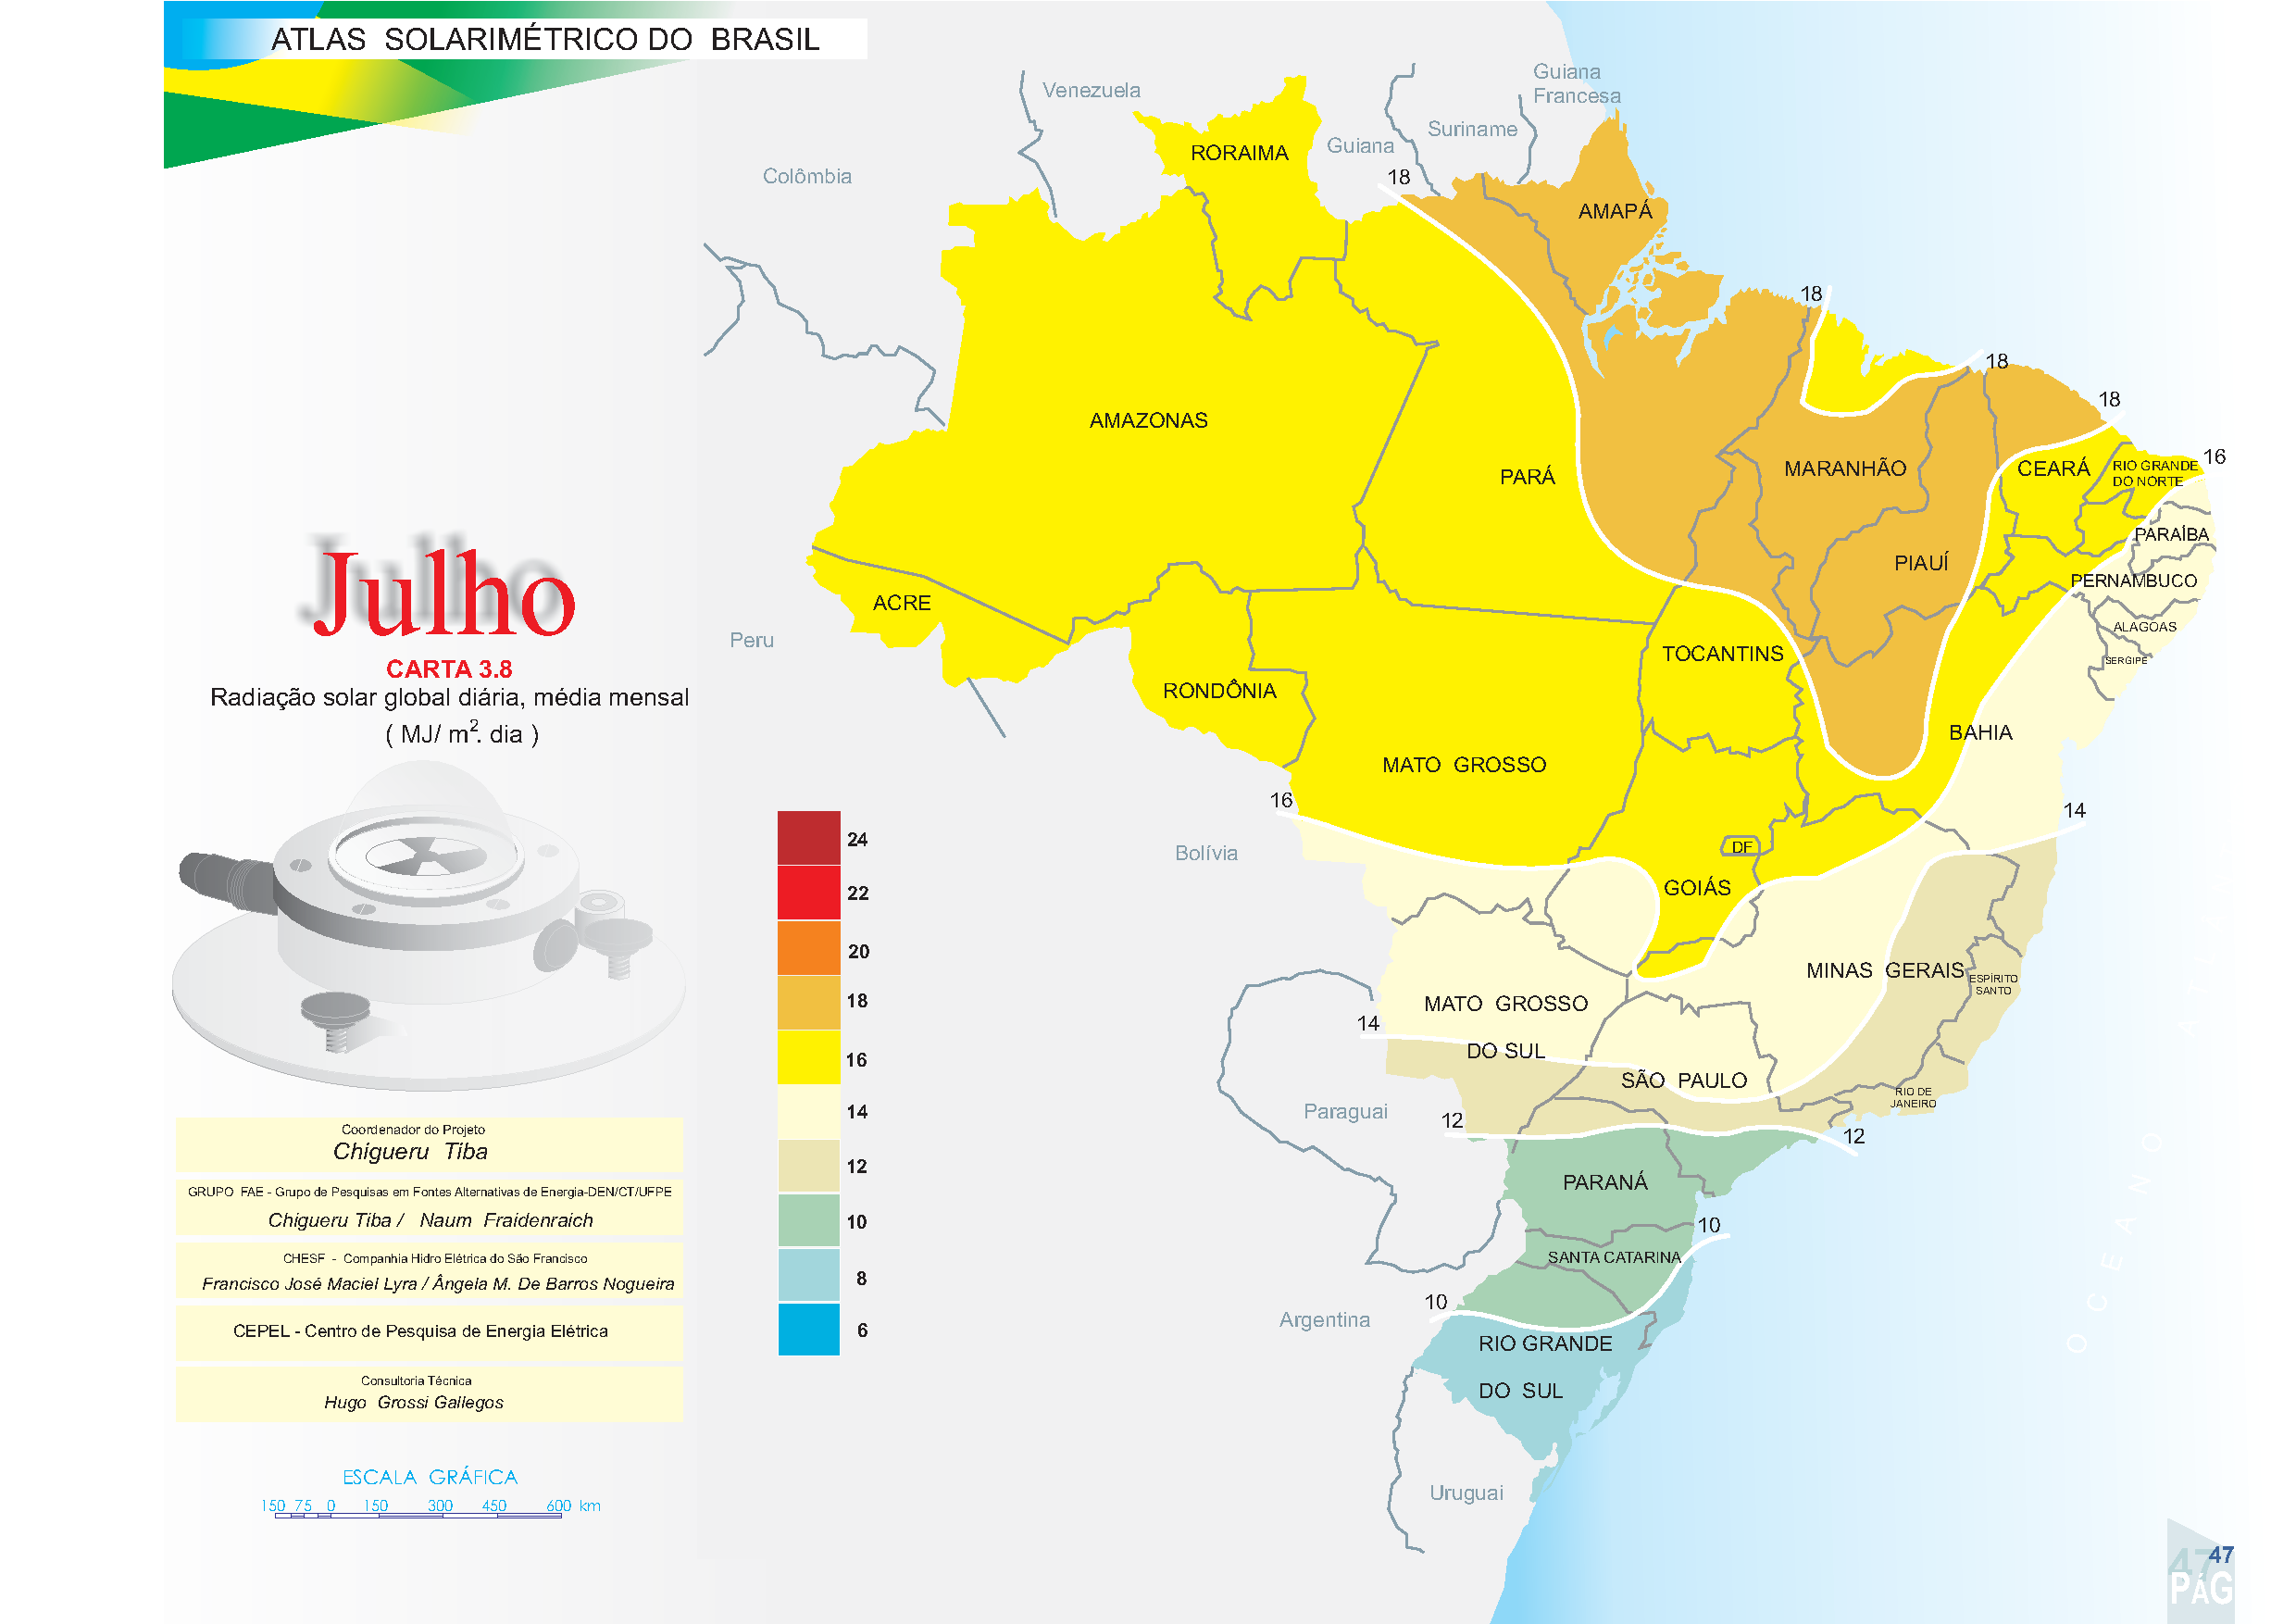
\includegraphics[scale=.12,center]{atlas_irra_jul}
    \end{column}
    \begin{column}{0.5\textwidth}
    	\centering
      	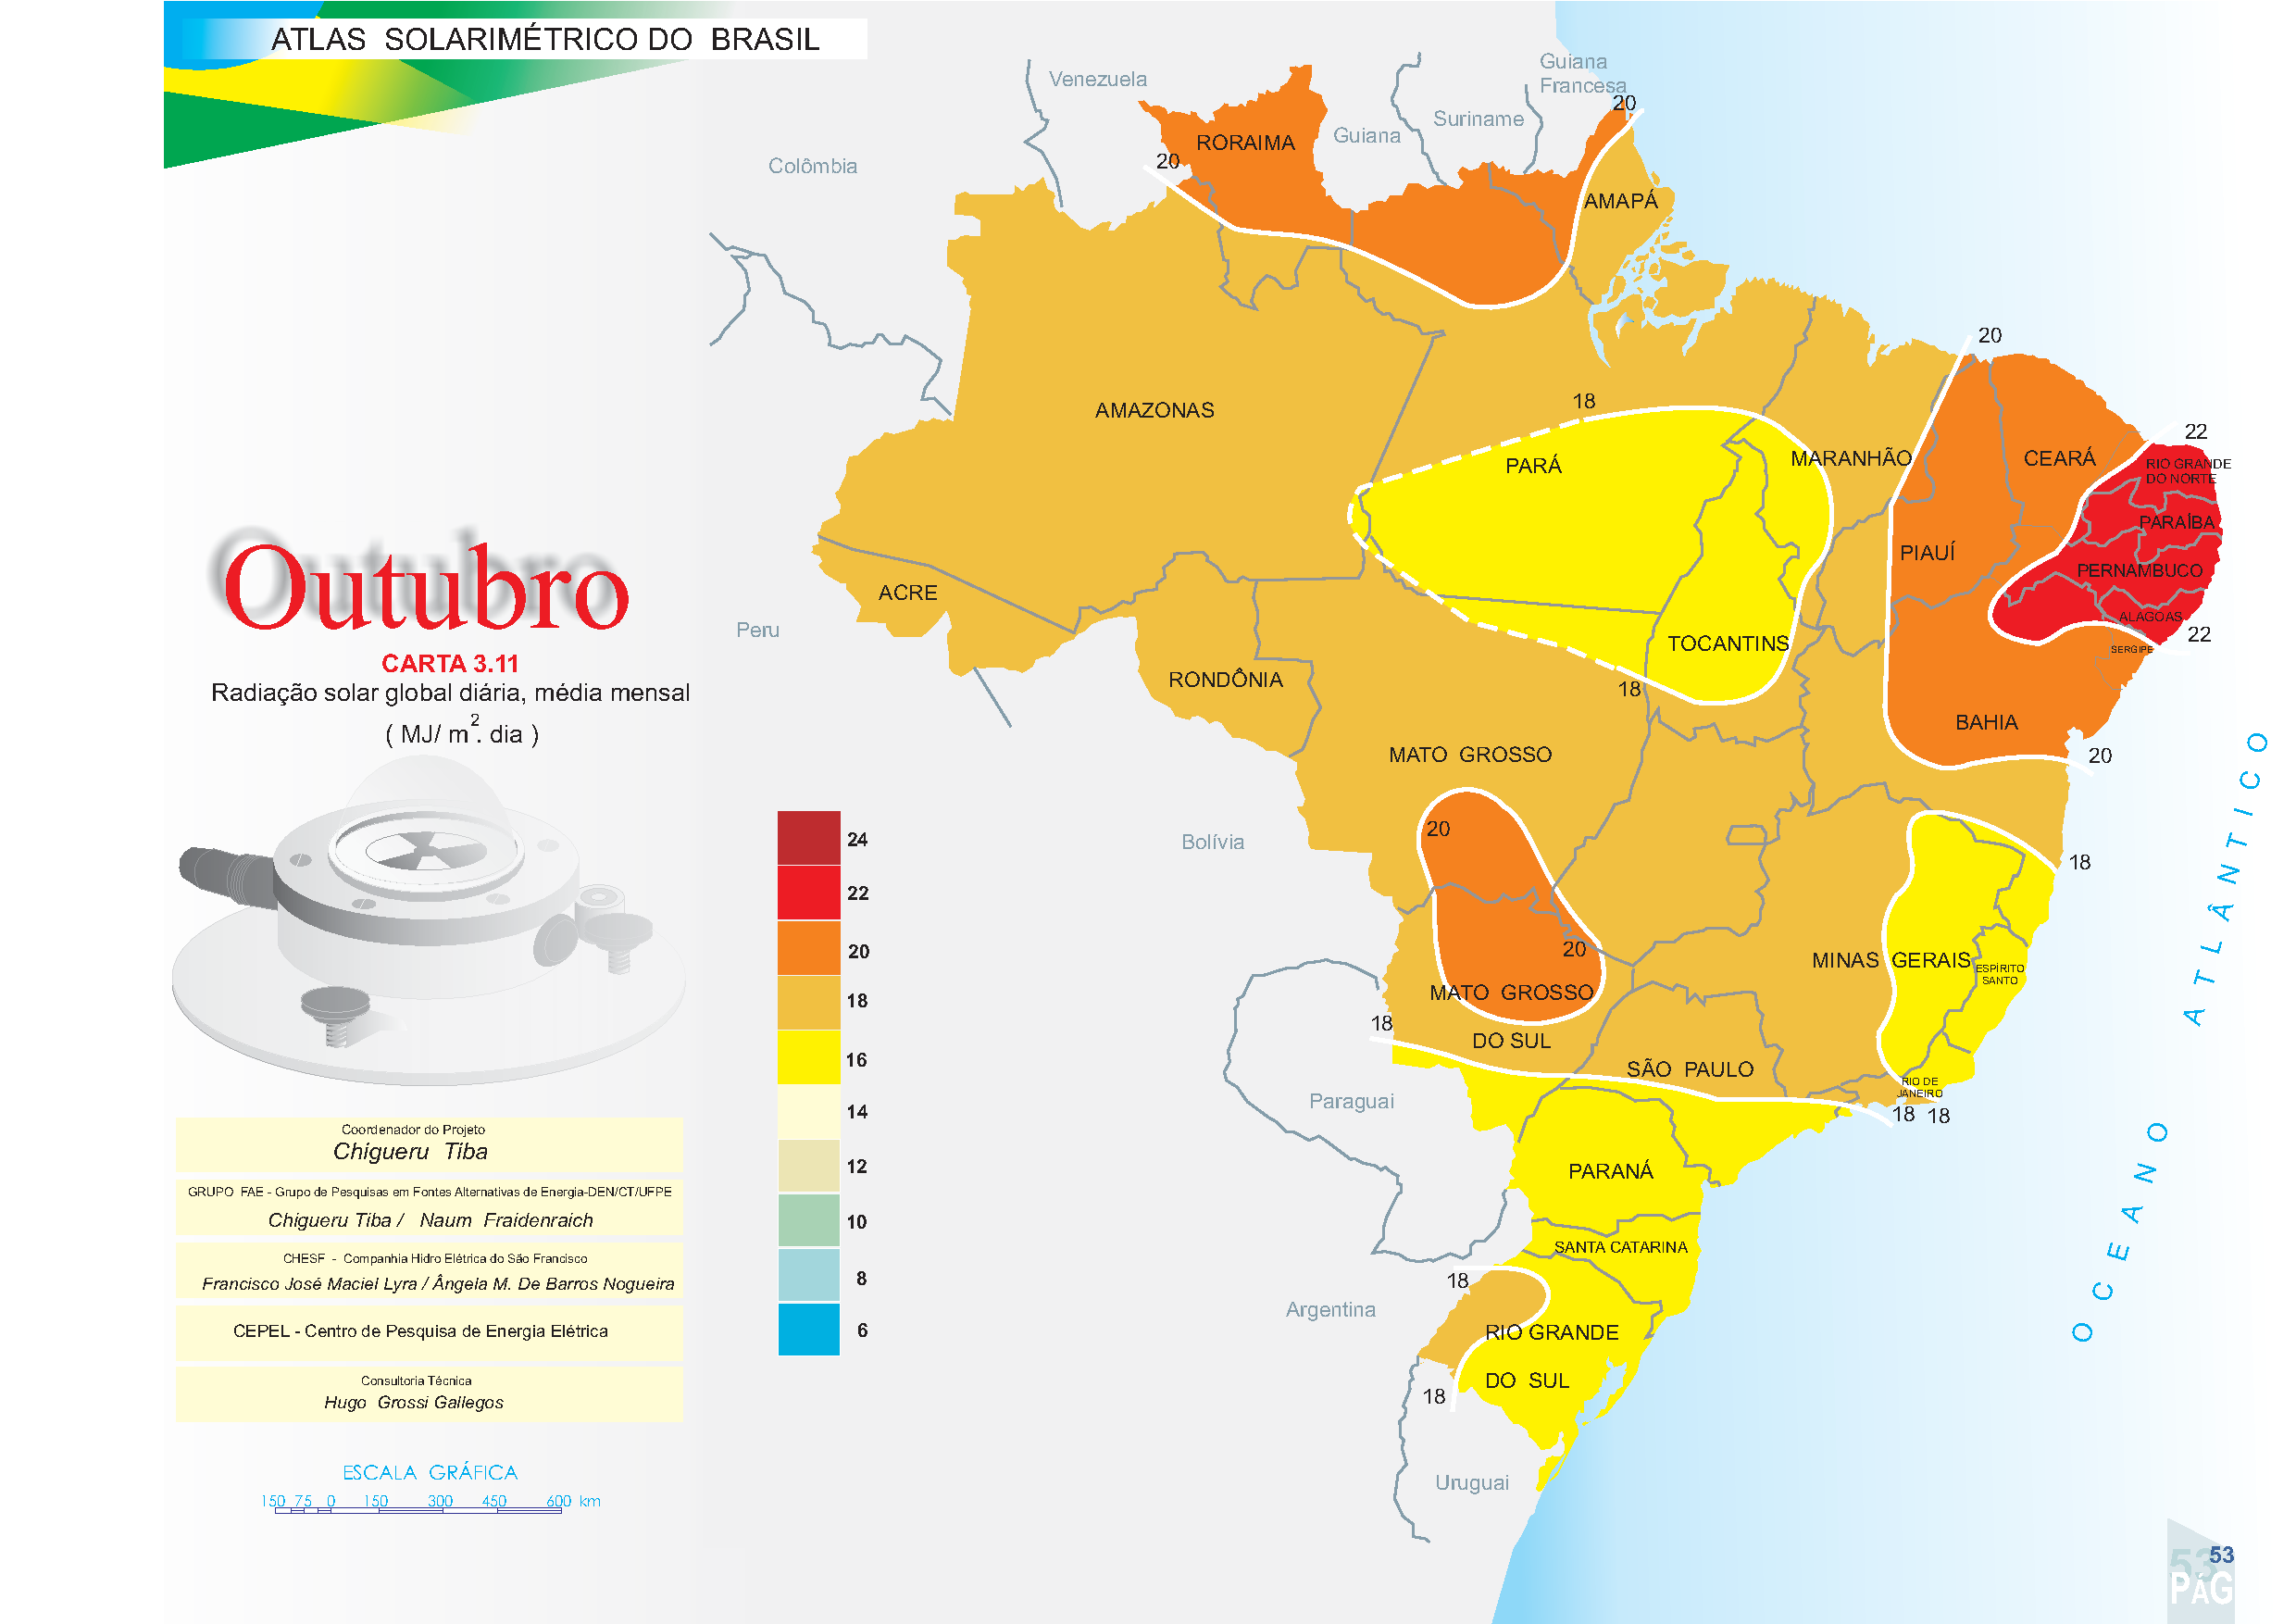
\includegraphics[scale=.12,center]{atlas_irra_out}
    \end{column}
\end{columns}

\end{frame}

\begin{frame}{Energia disponível no local}

\begin{figure}[H]
	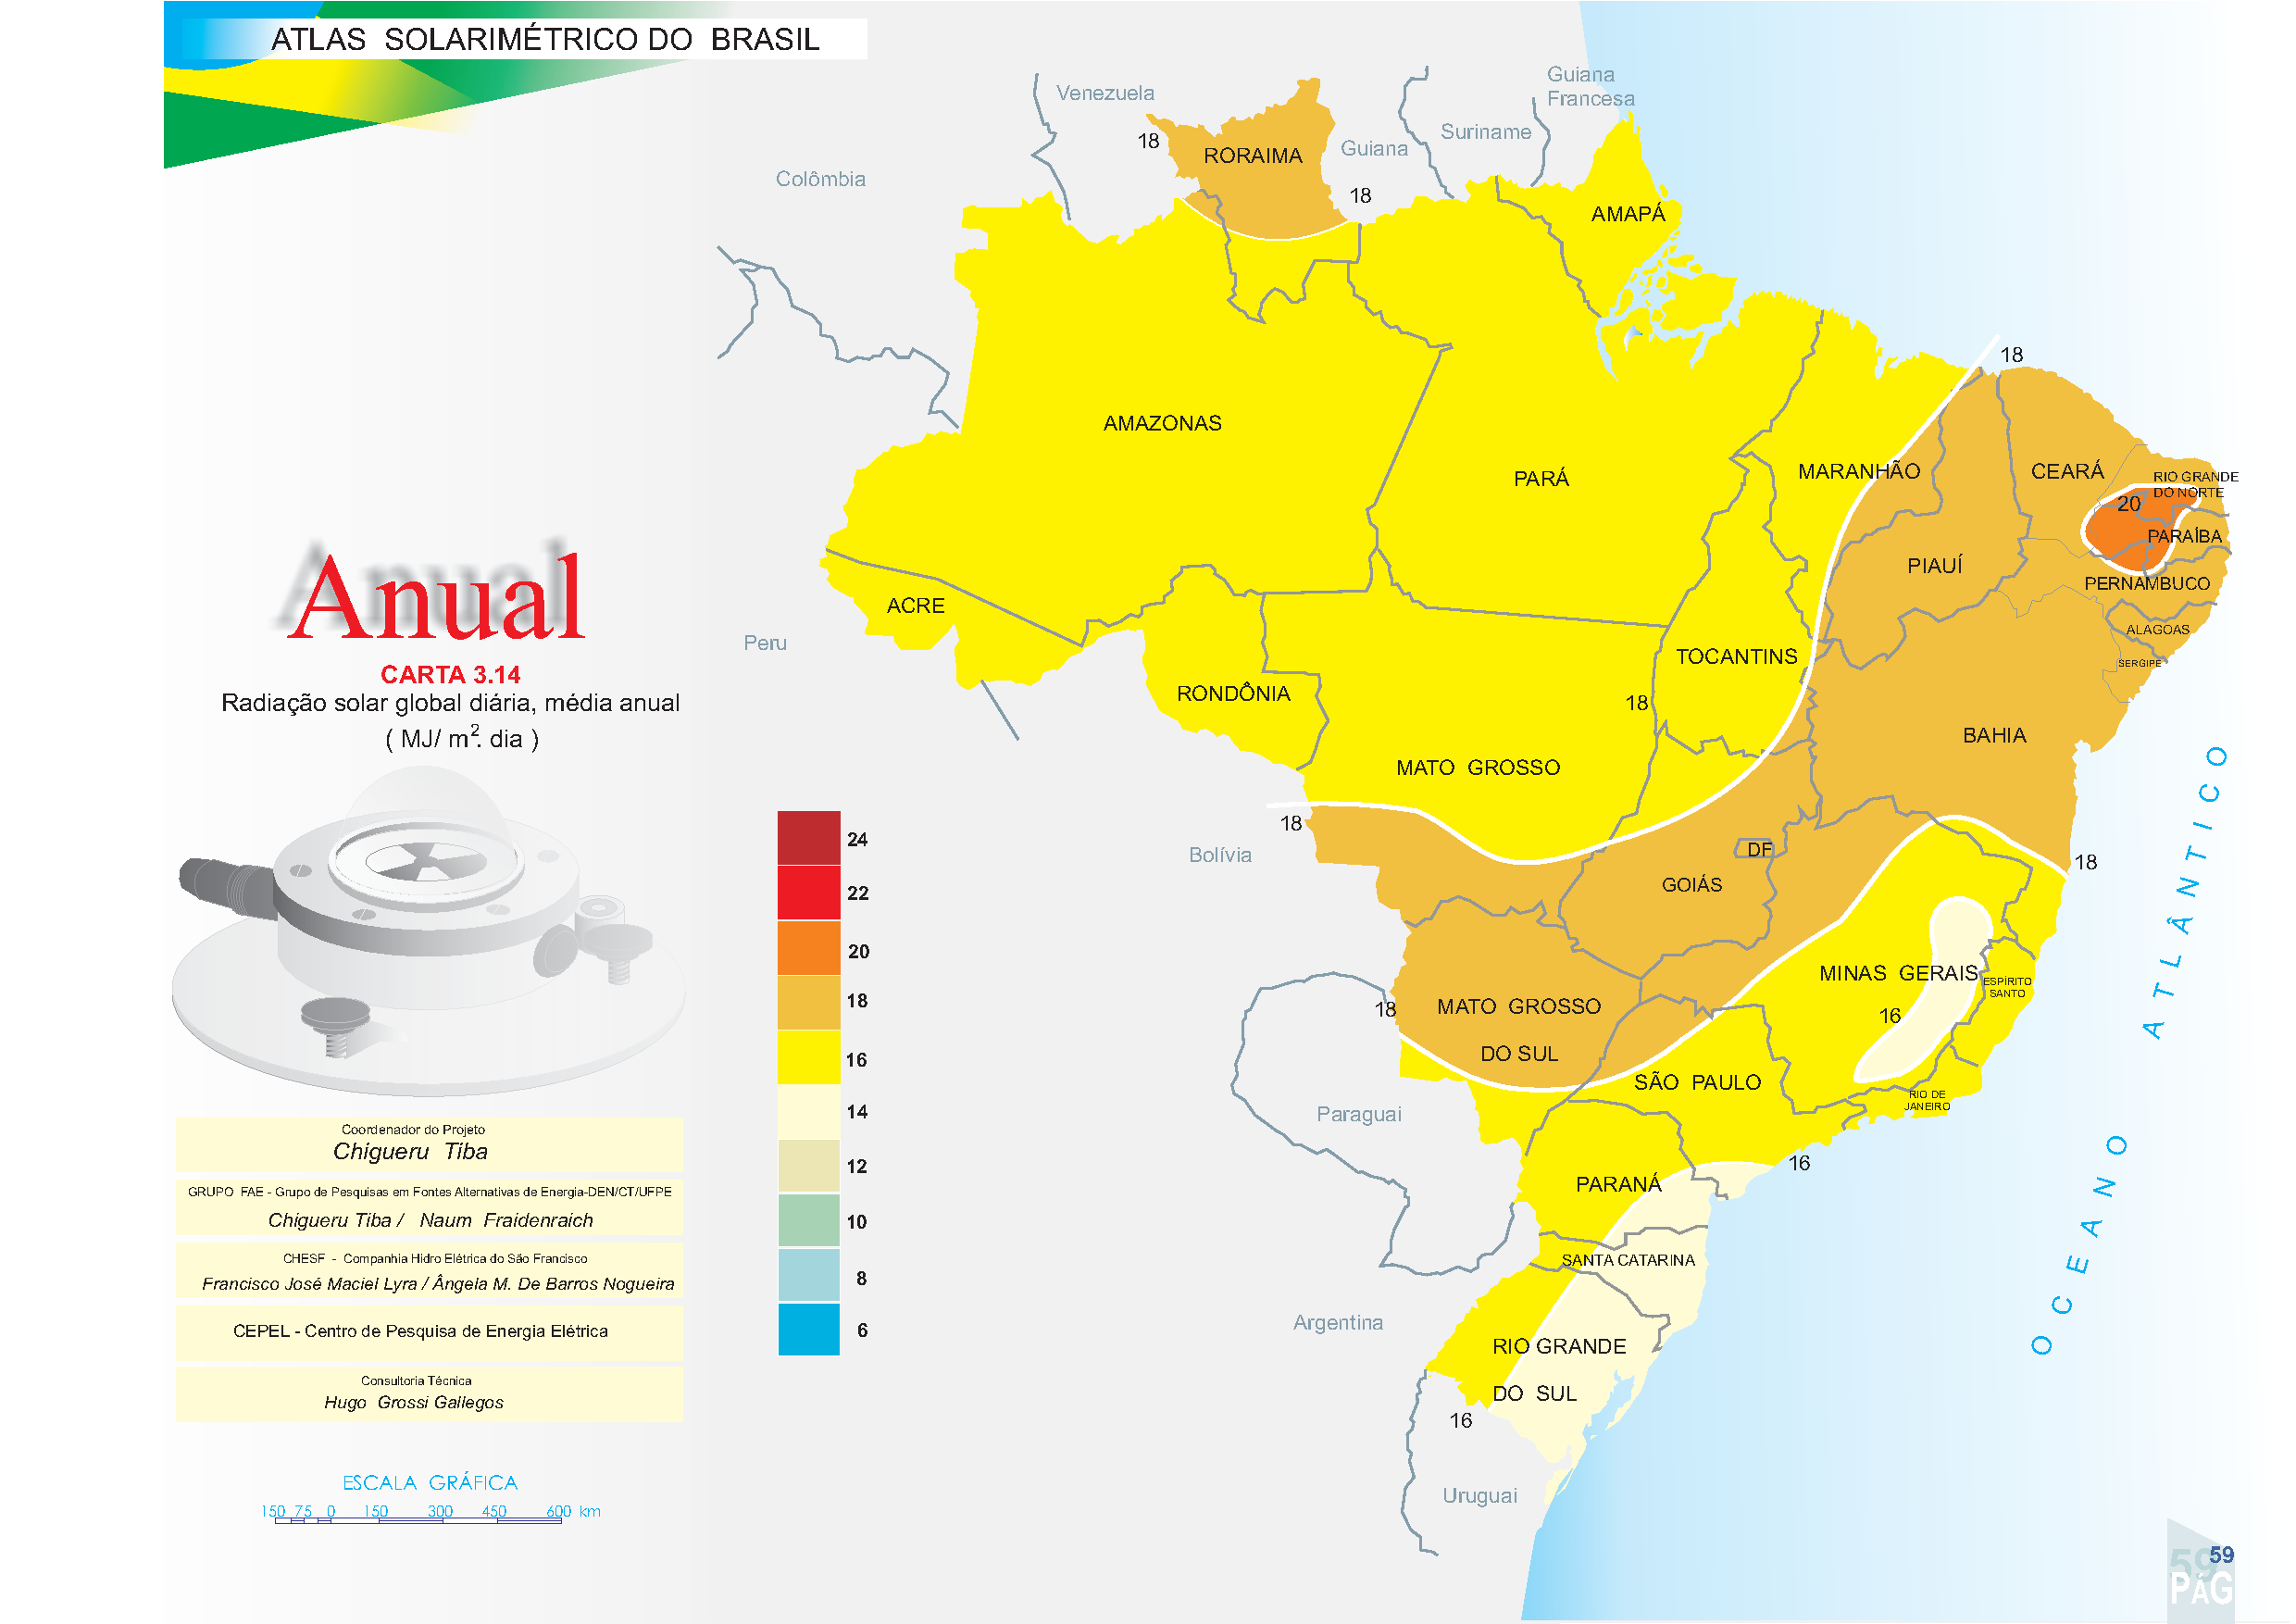
\includegraphics[scale=.25,center]{atlas_irra_ano}
\end{figure}

\end{frame}

\begin{frame}{Energia disponível no local}

\begin{columns}[T]
    \begin{column}{0.5\textwidth}
    	\centering
      	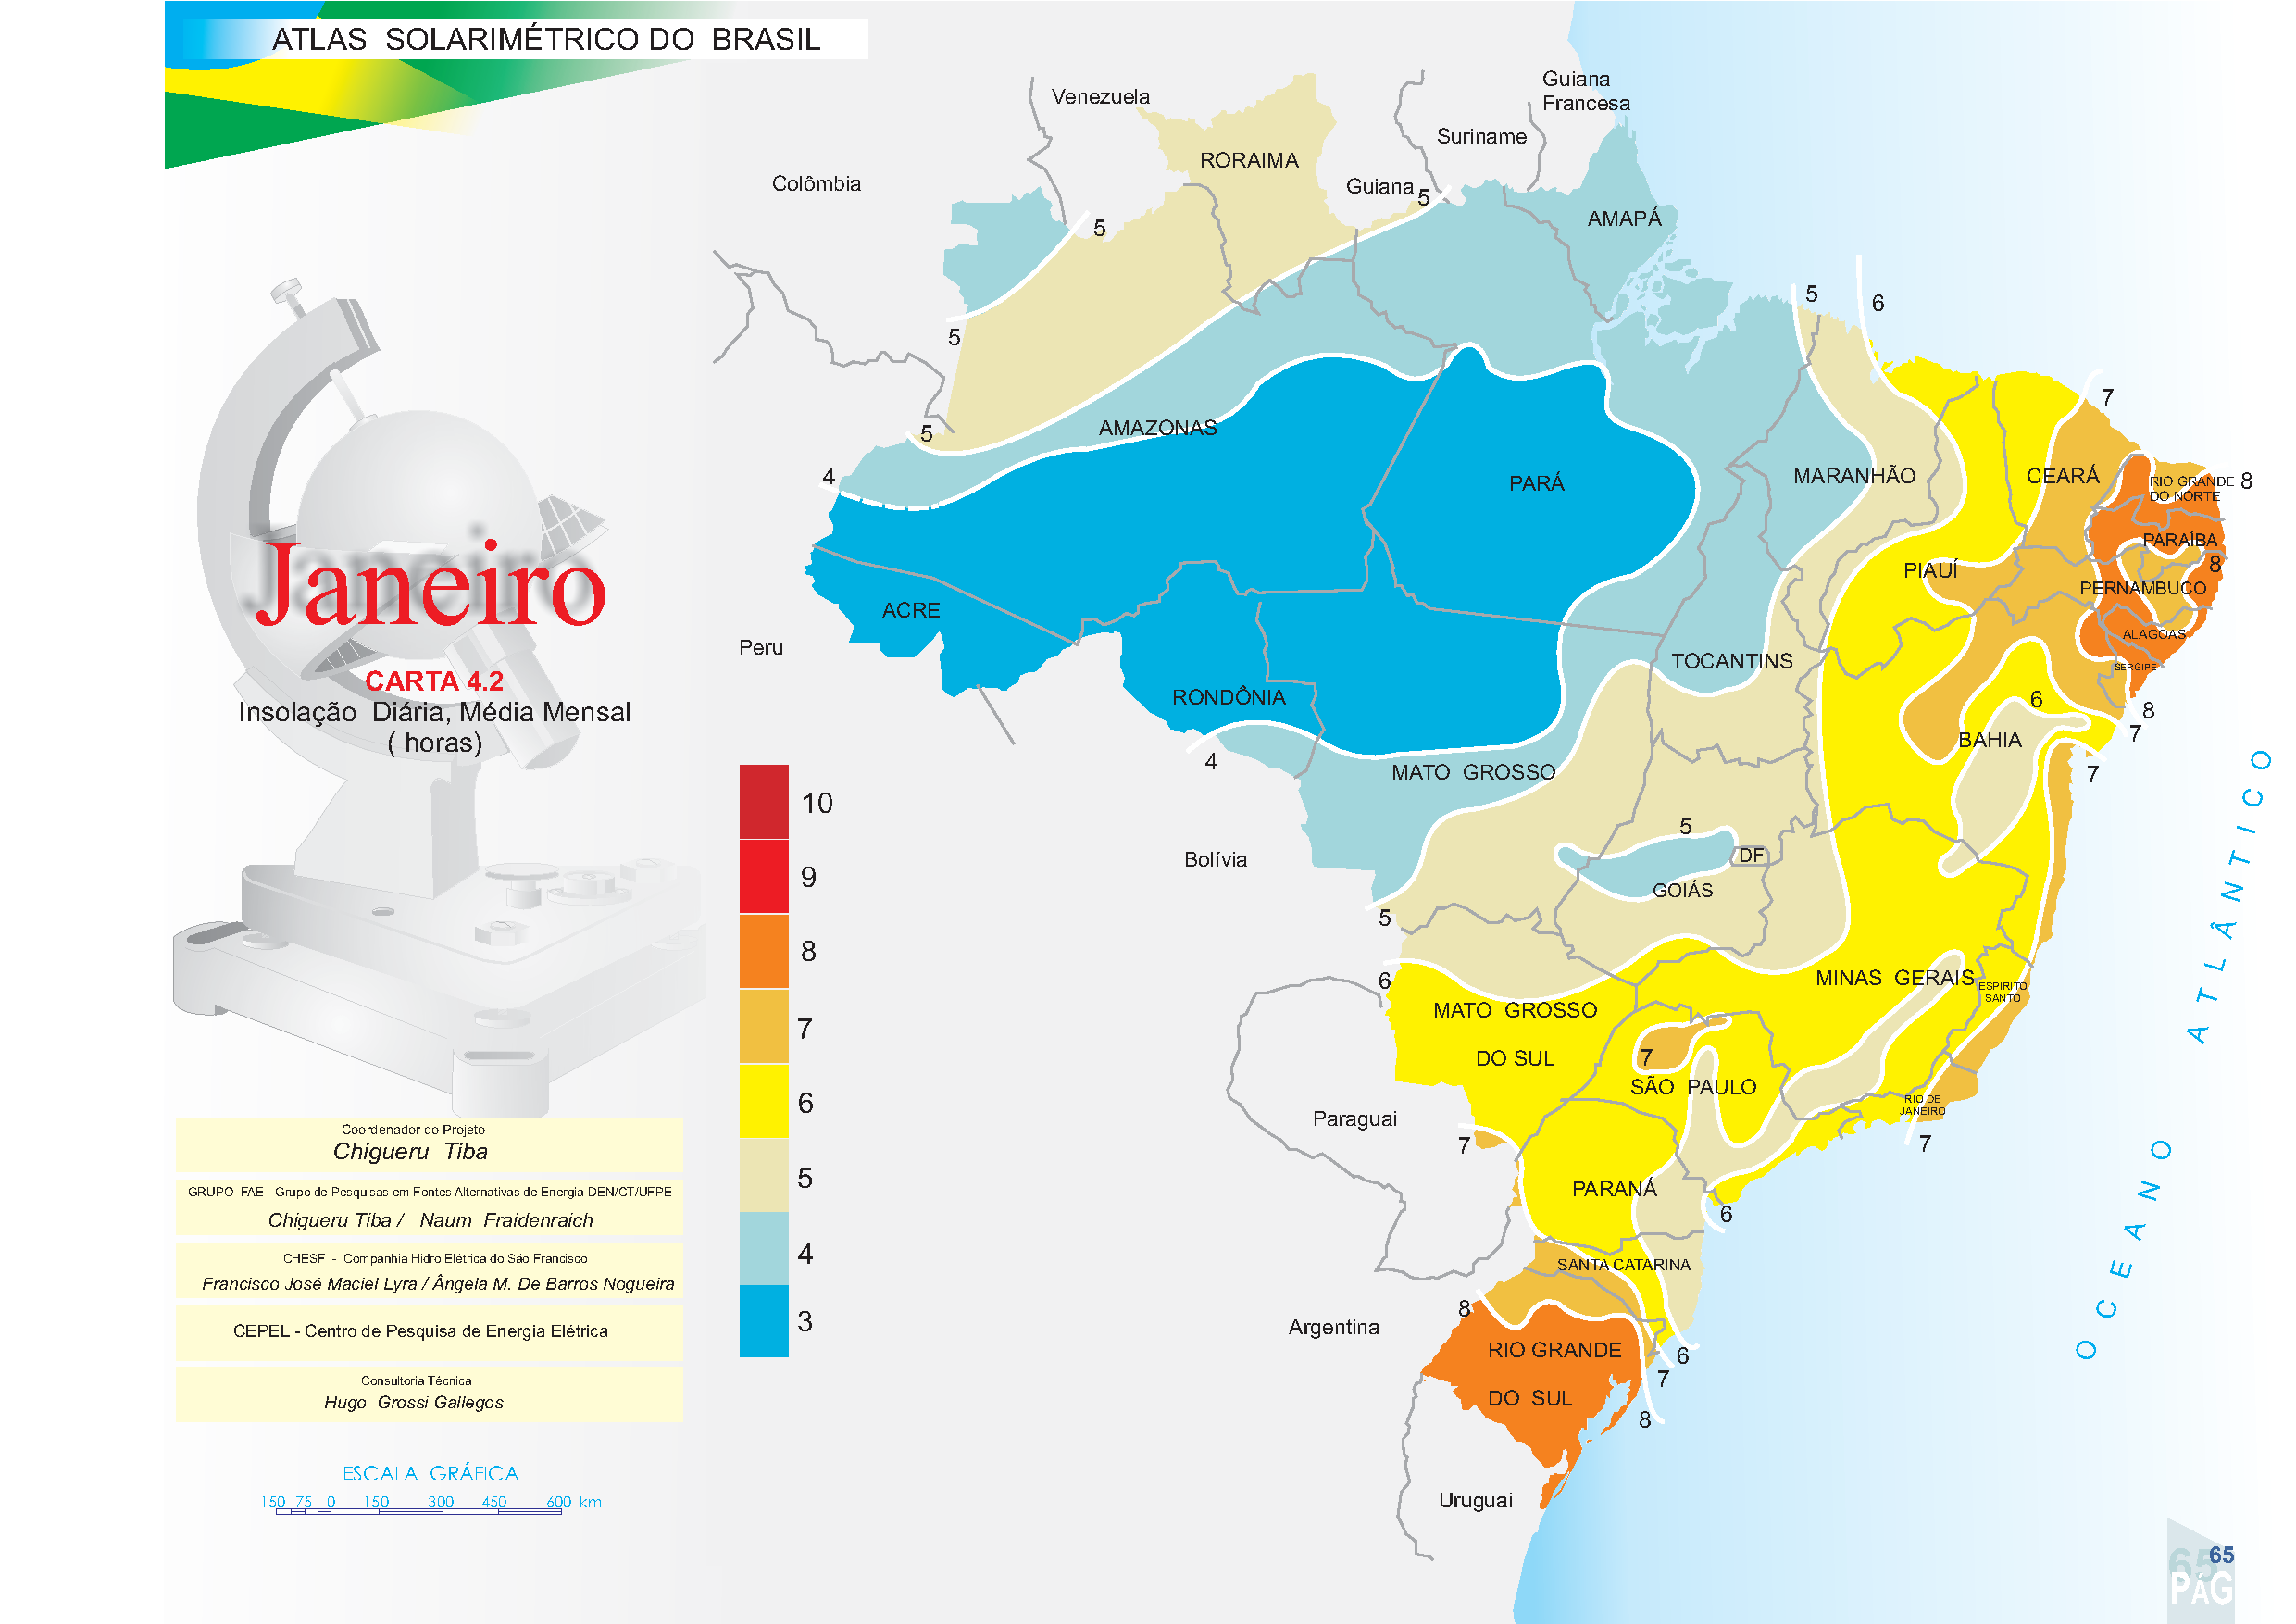
\includegraphics[scale=.12,center]{atlas_inso_jan}
    \end{column}
    \begin{column}{0.5\textwidth}
    	\centering
      	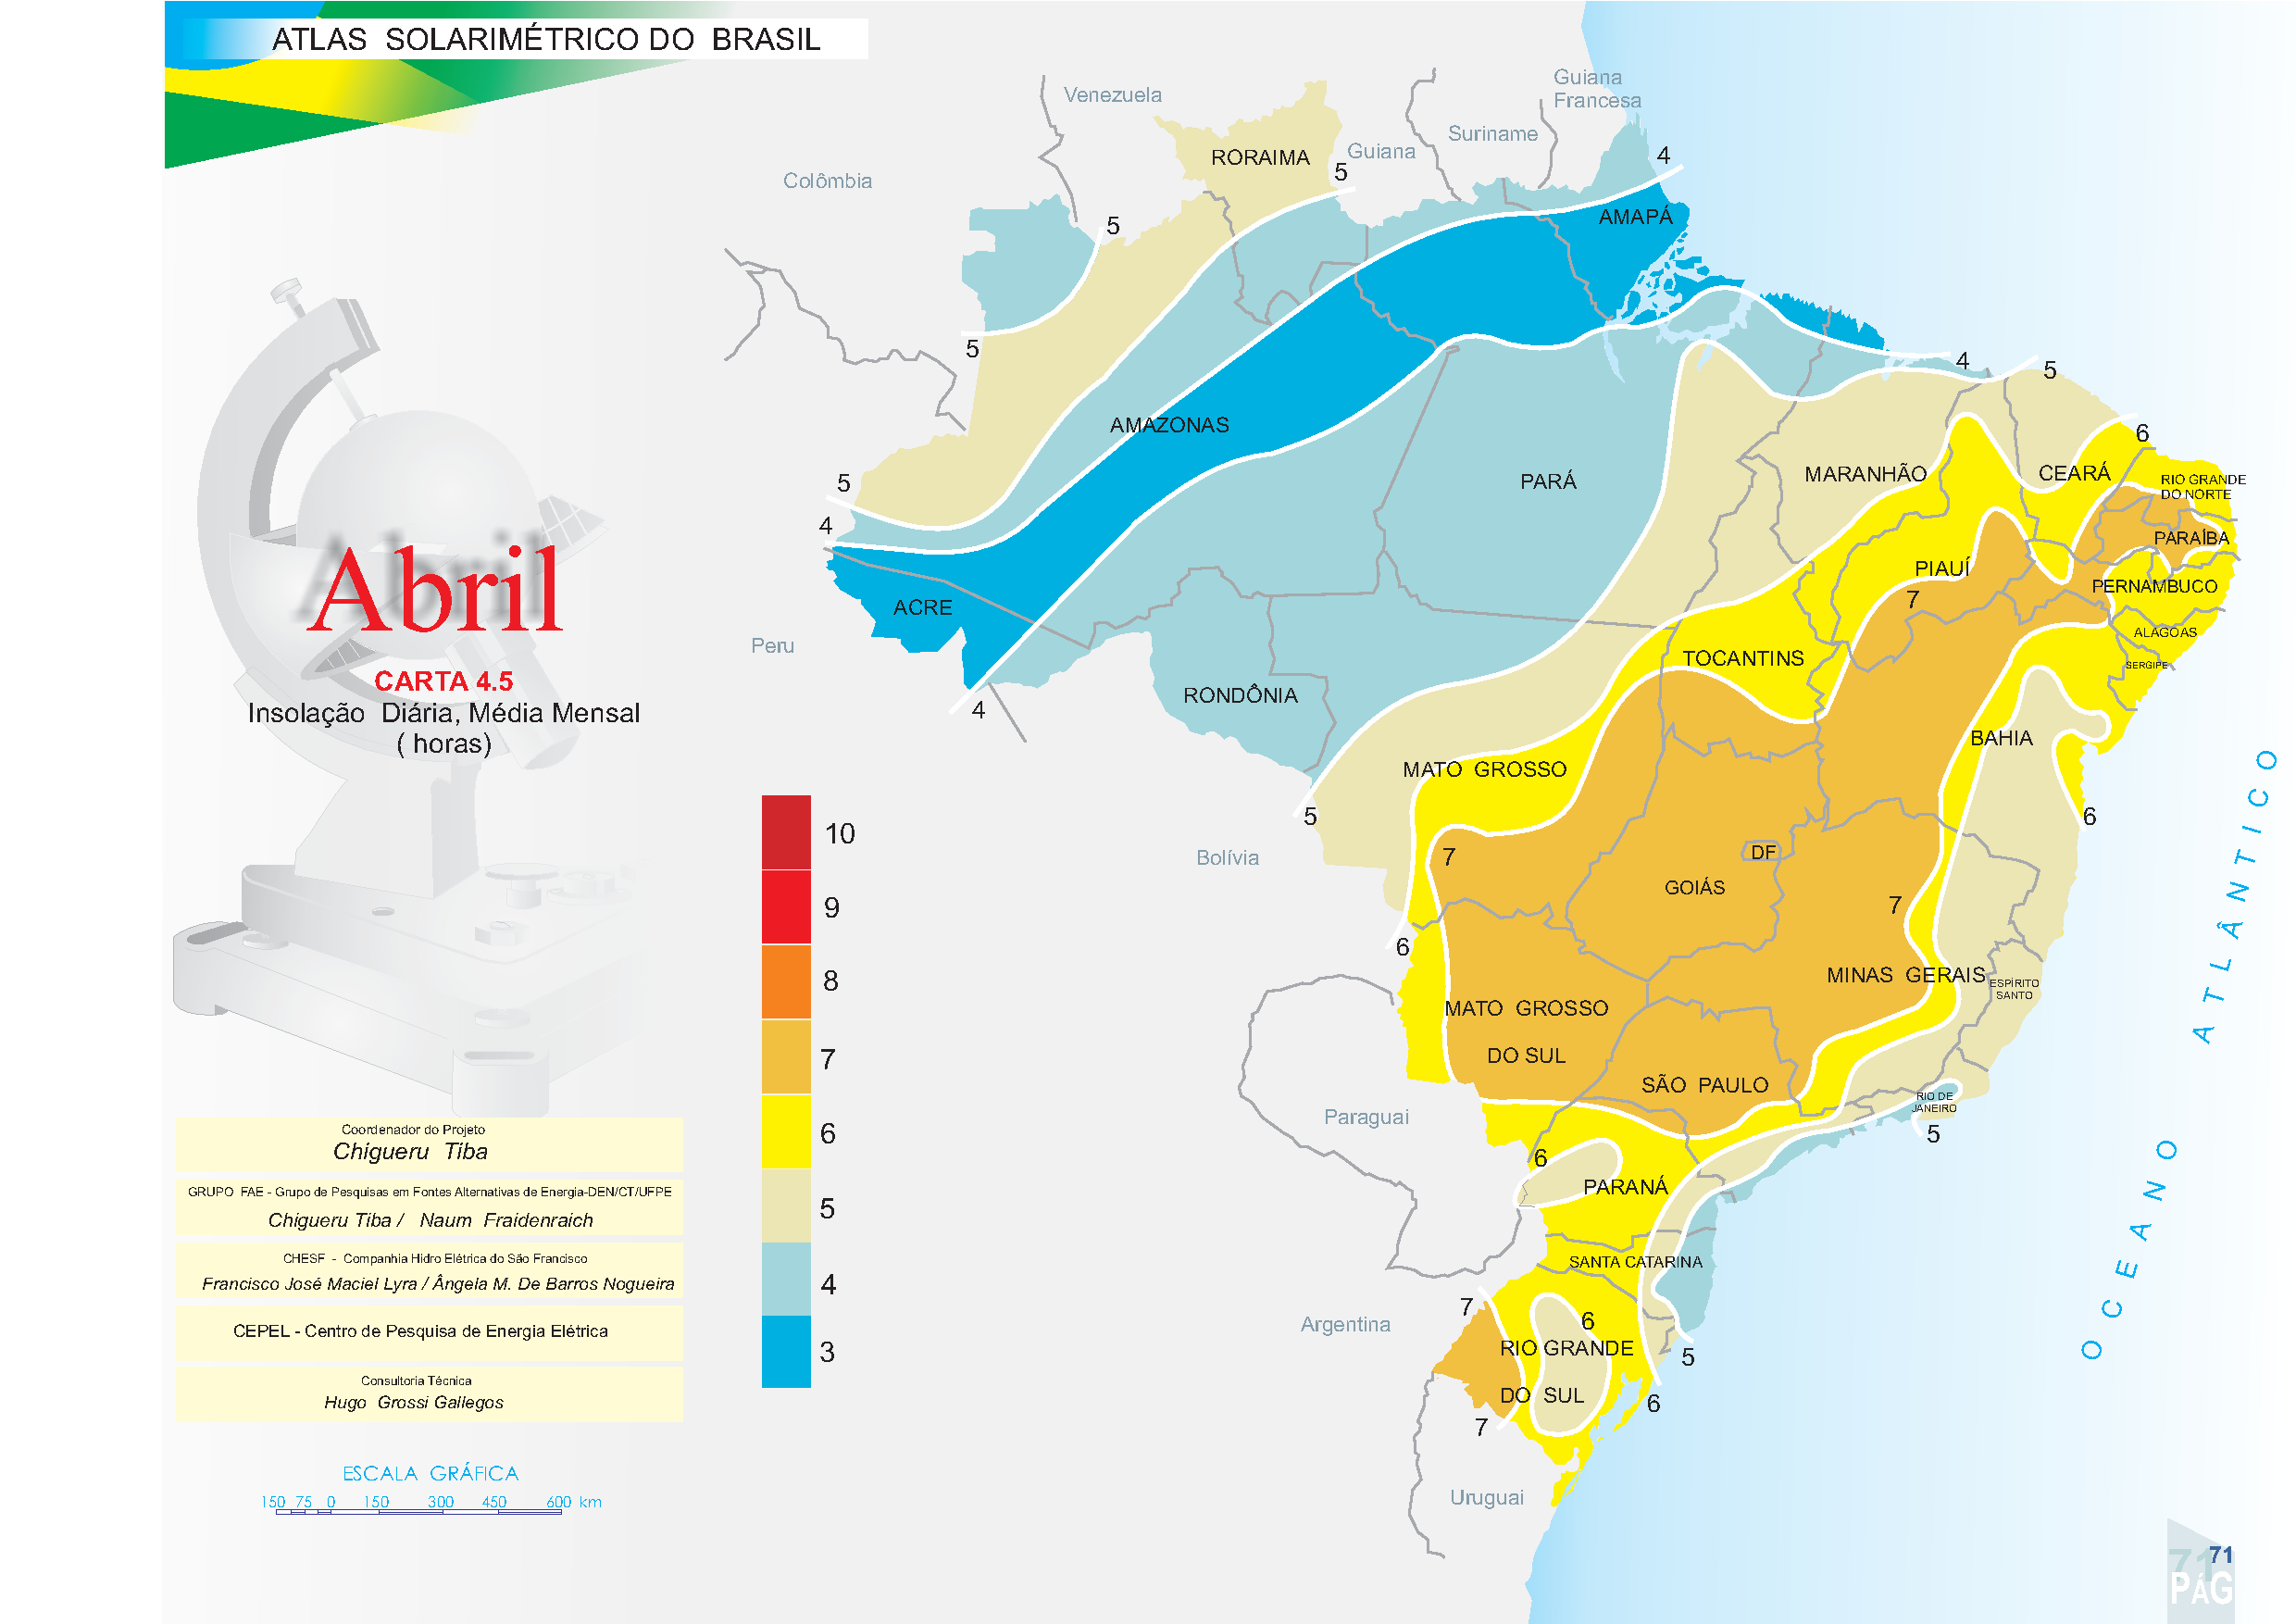
\includegraphics[scale=.12,center]{atlas_inso_abr}
    \end{column}
\end{columns}

\vspace{.25cm}

\begin{columns}[T]
    \begin{column}{0.5\textwidth}
    	\centering
      	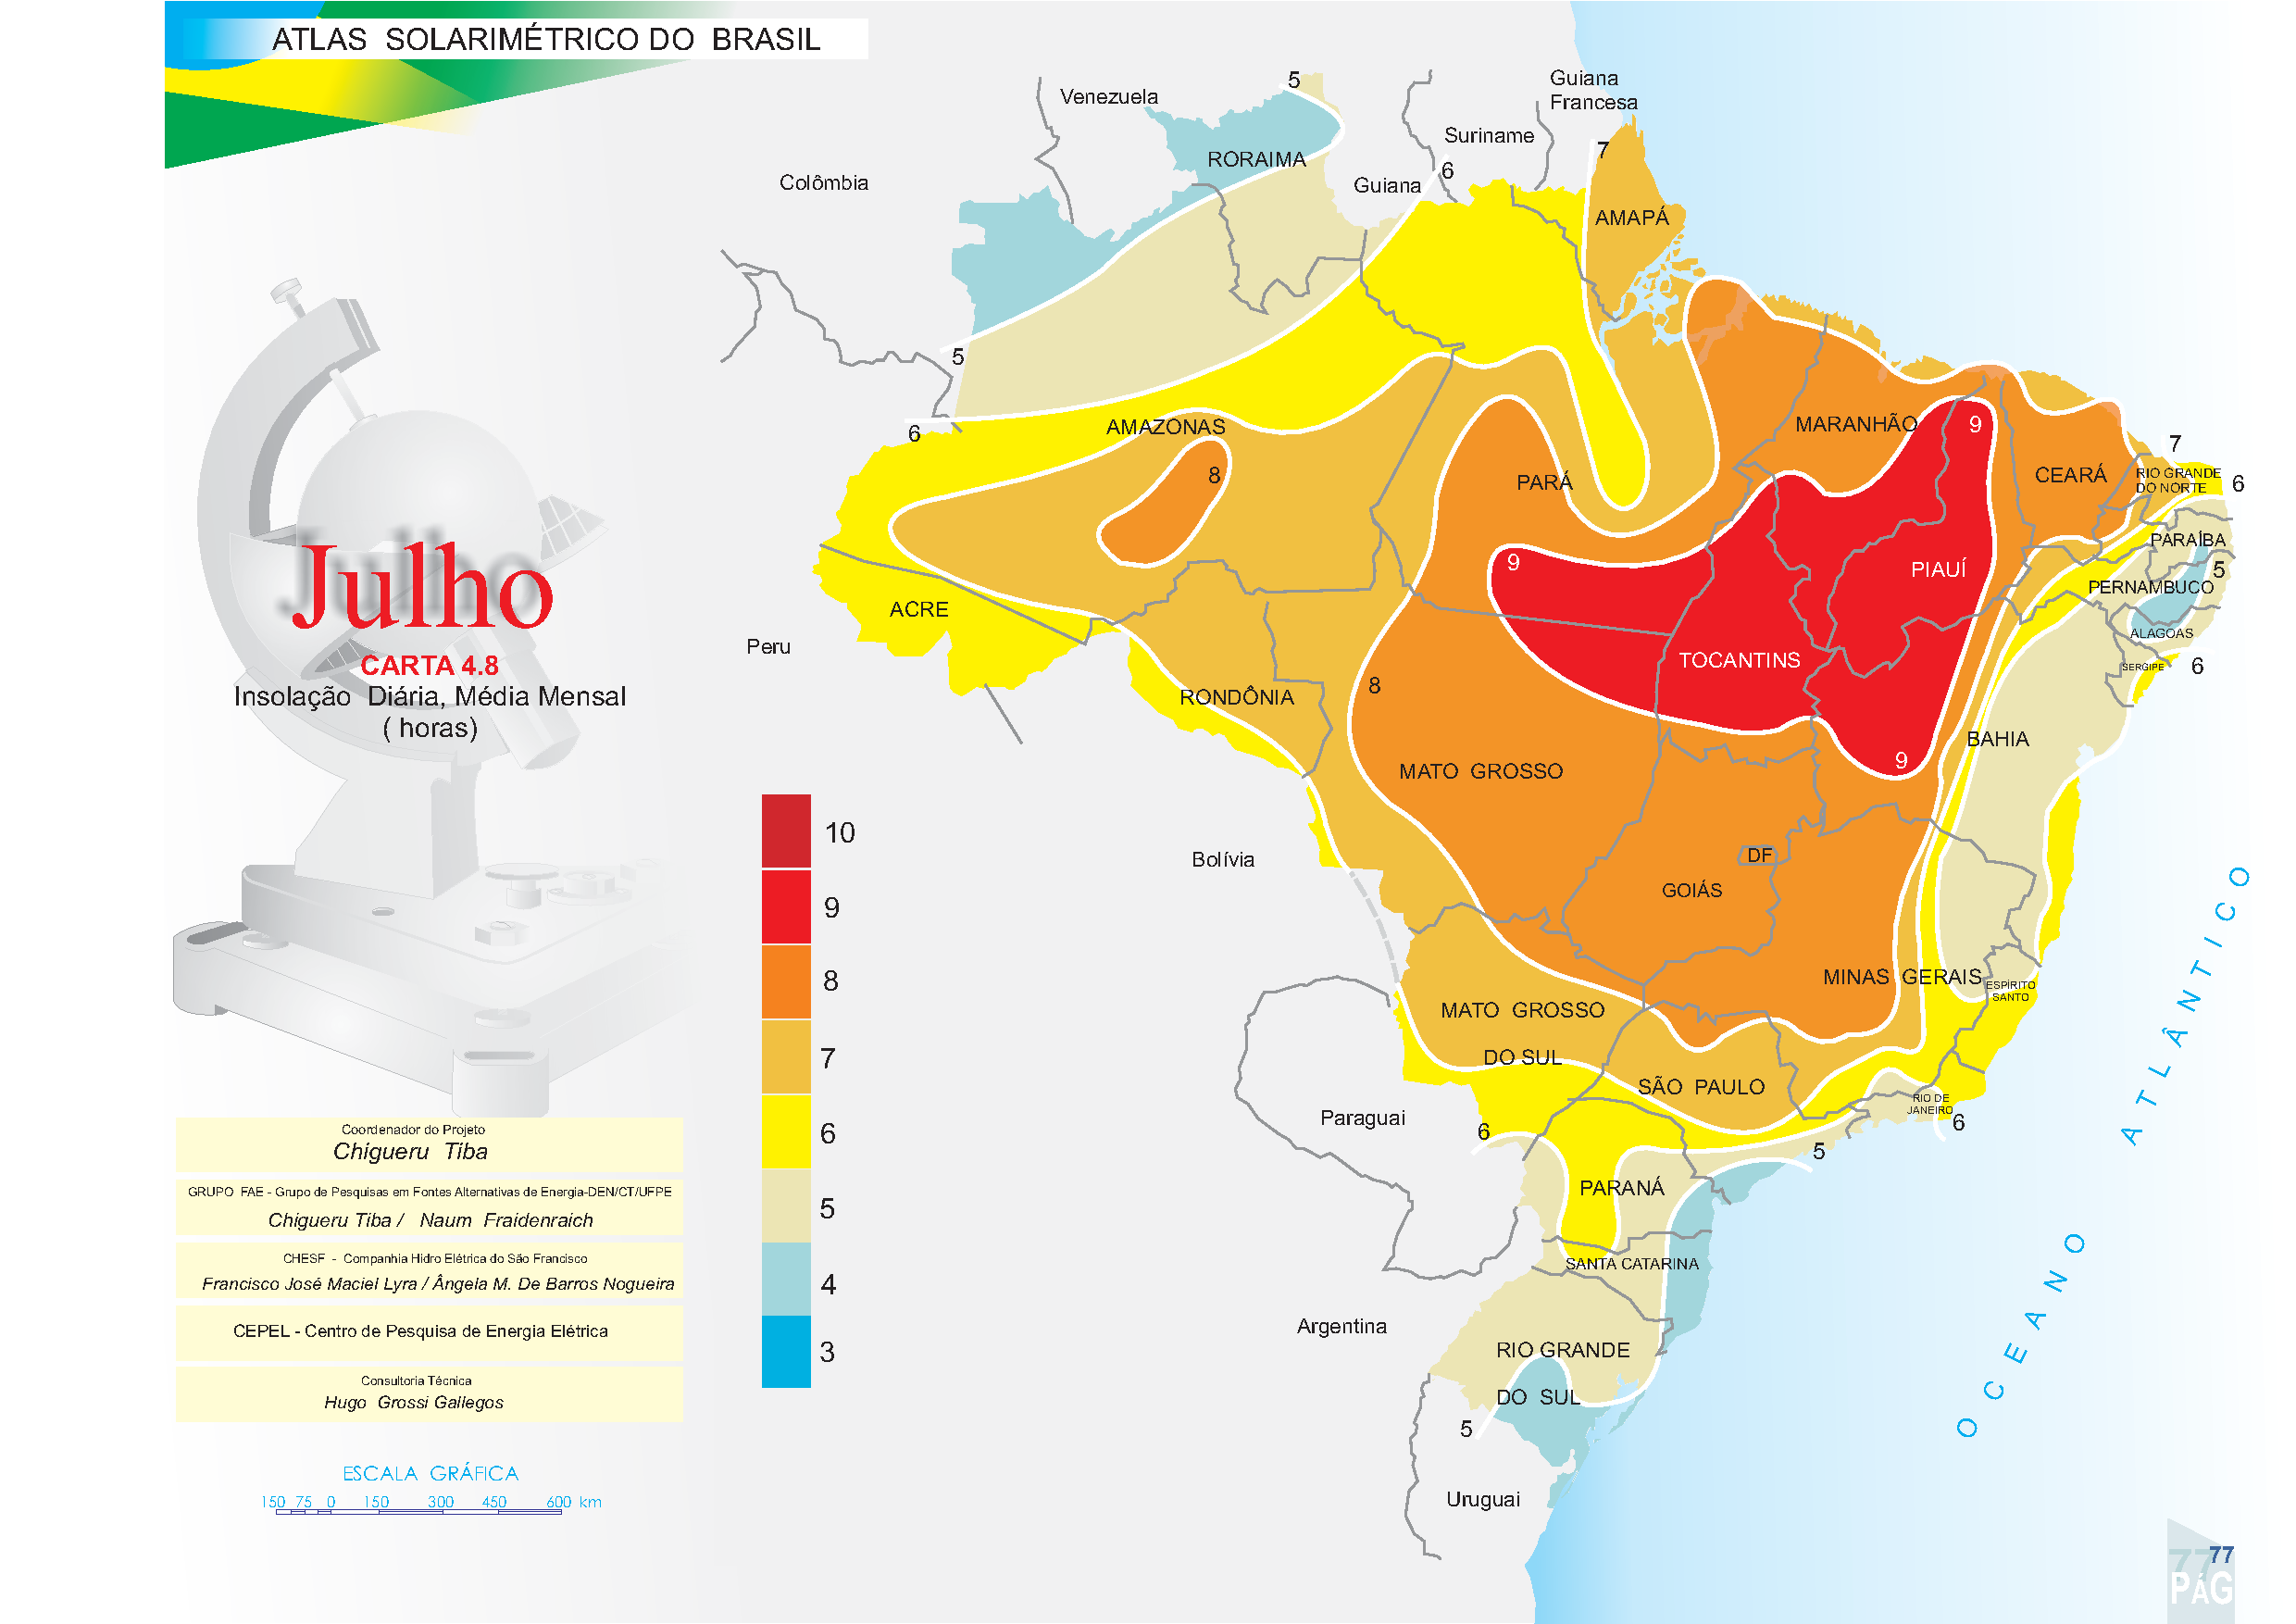
\includegraphics[scale=.12,center]{atlas_inso_jul}
    \end{column}
    \begin{column}{0.5\textwidth}
    	\centering
      	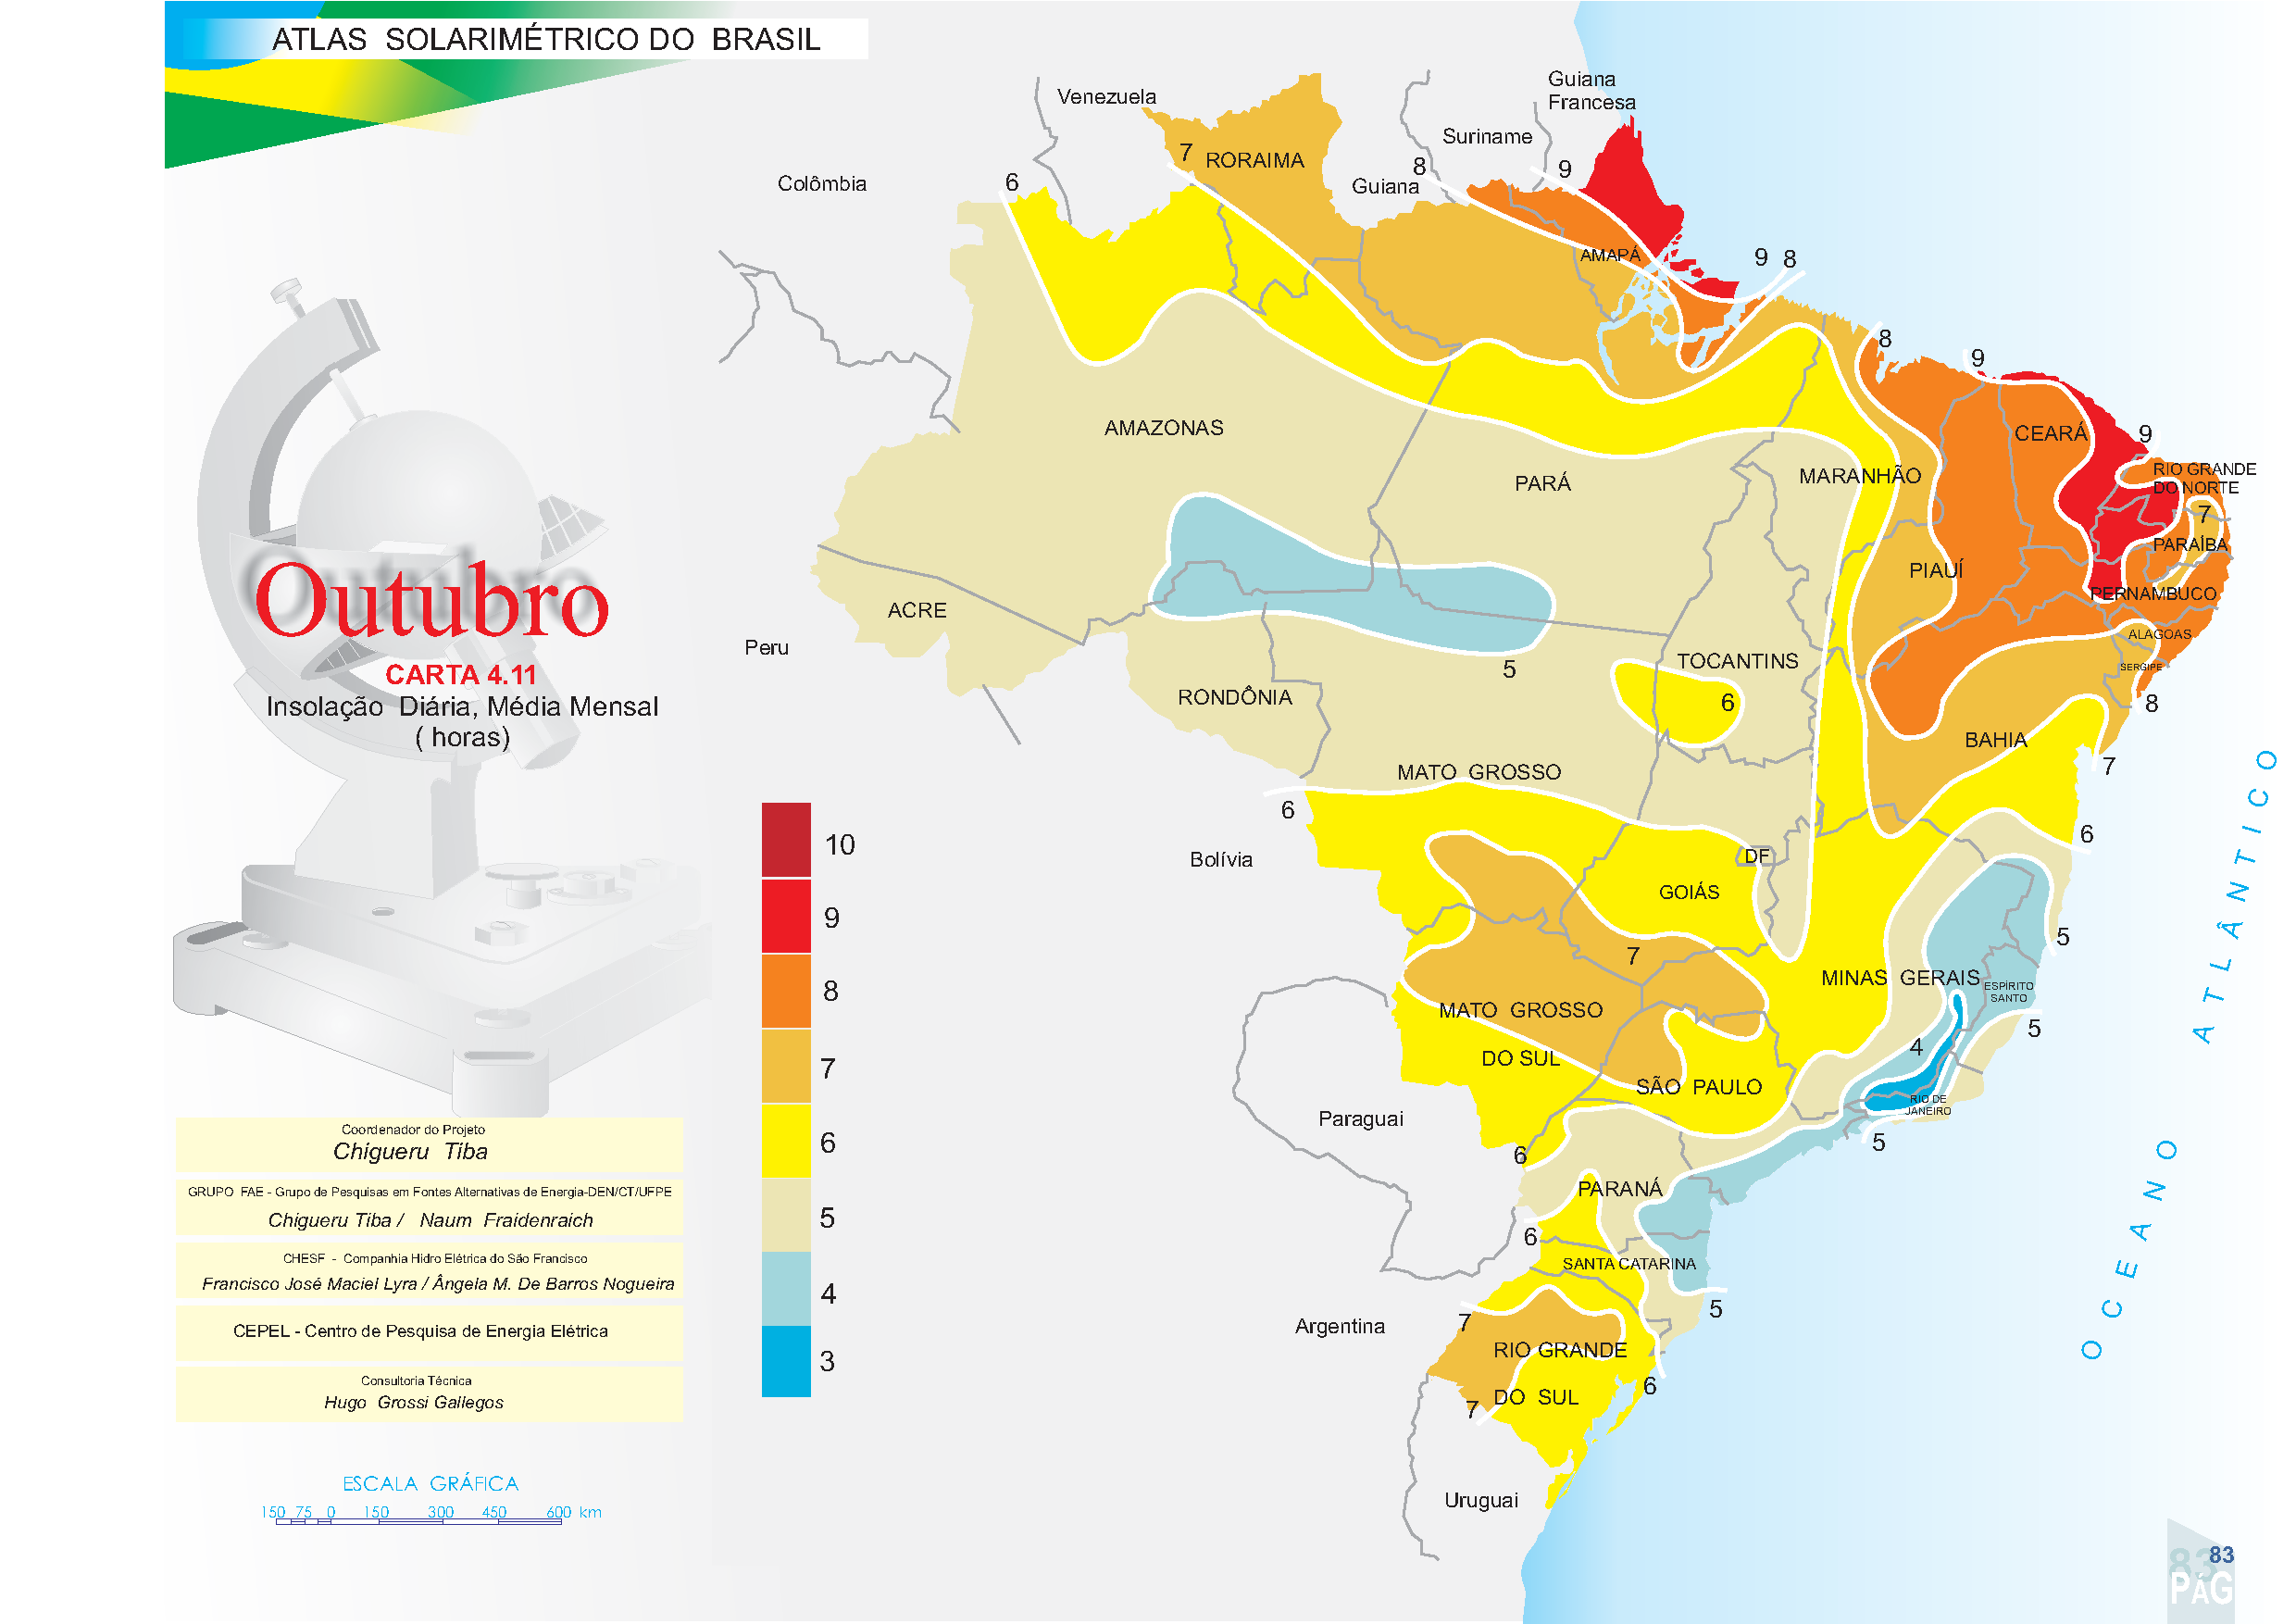
\includegraphics[scale=.12,center]{atlas_inso_out}
    \end{column}
\end{columns}

\end{frame}

\begin{frame}{Energia disponível no local}

\begin{figure}[H]
	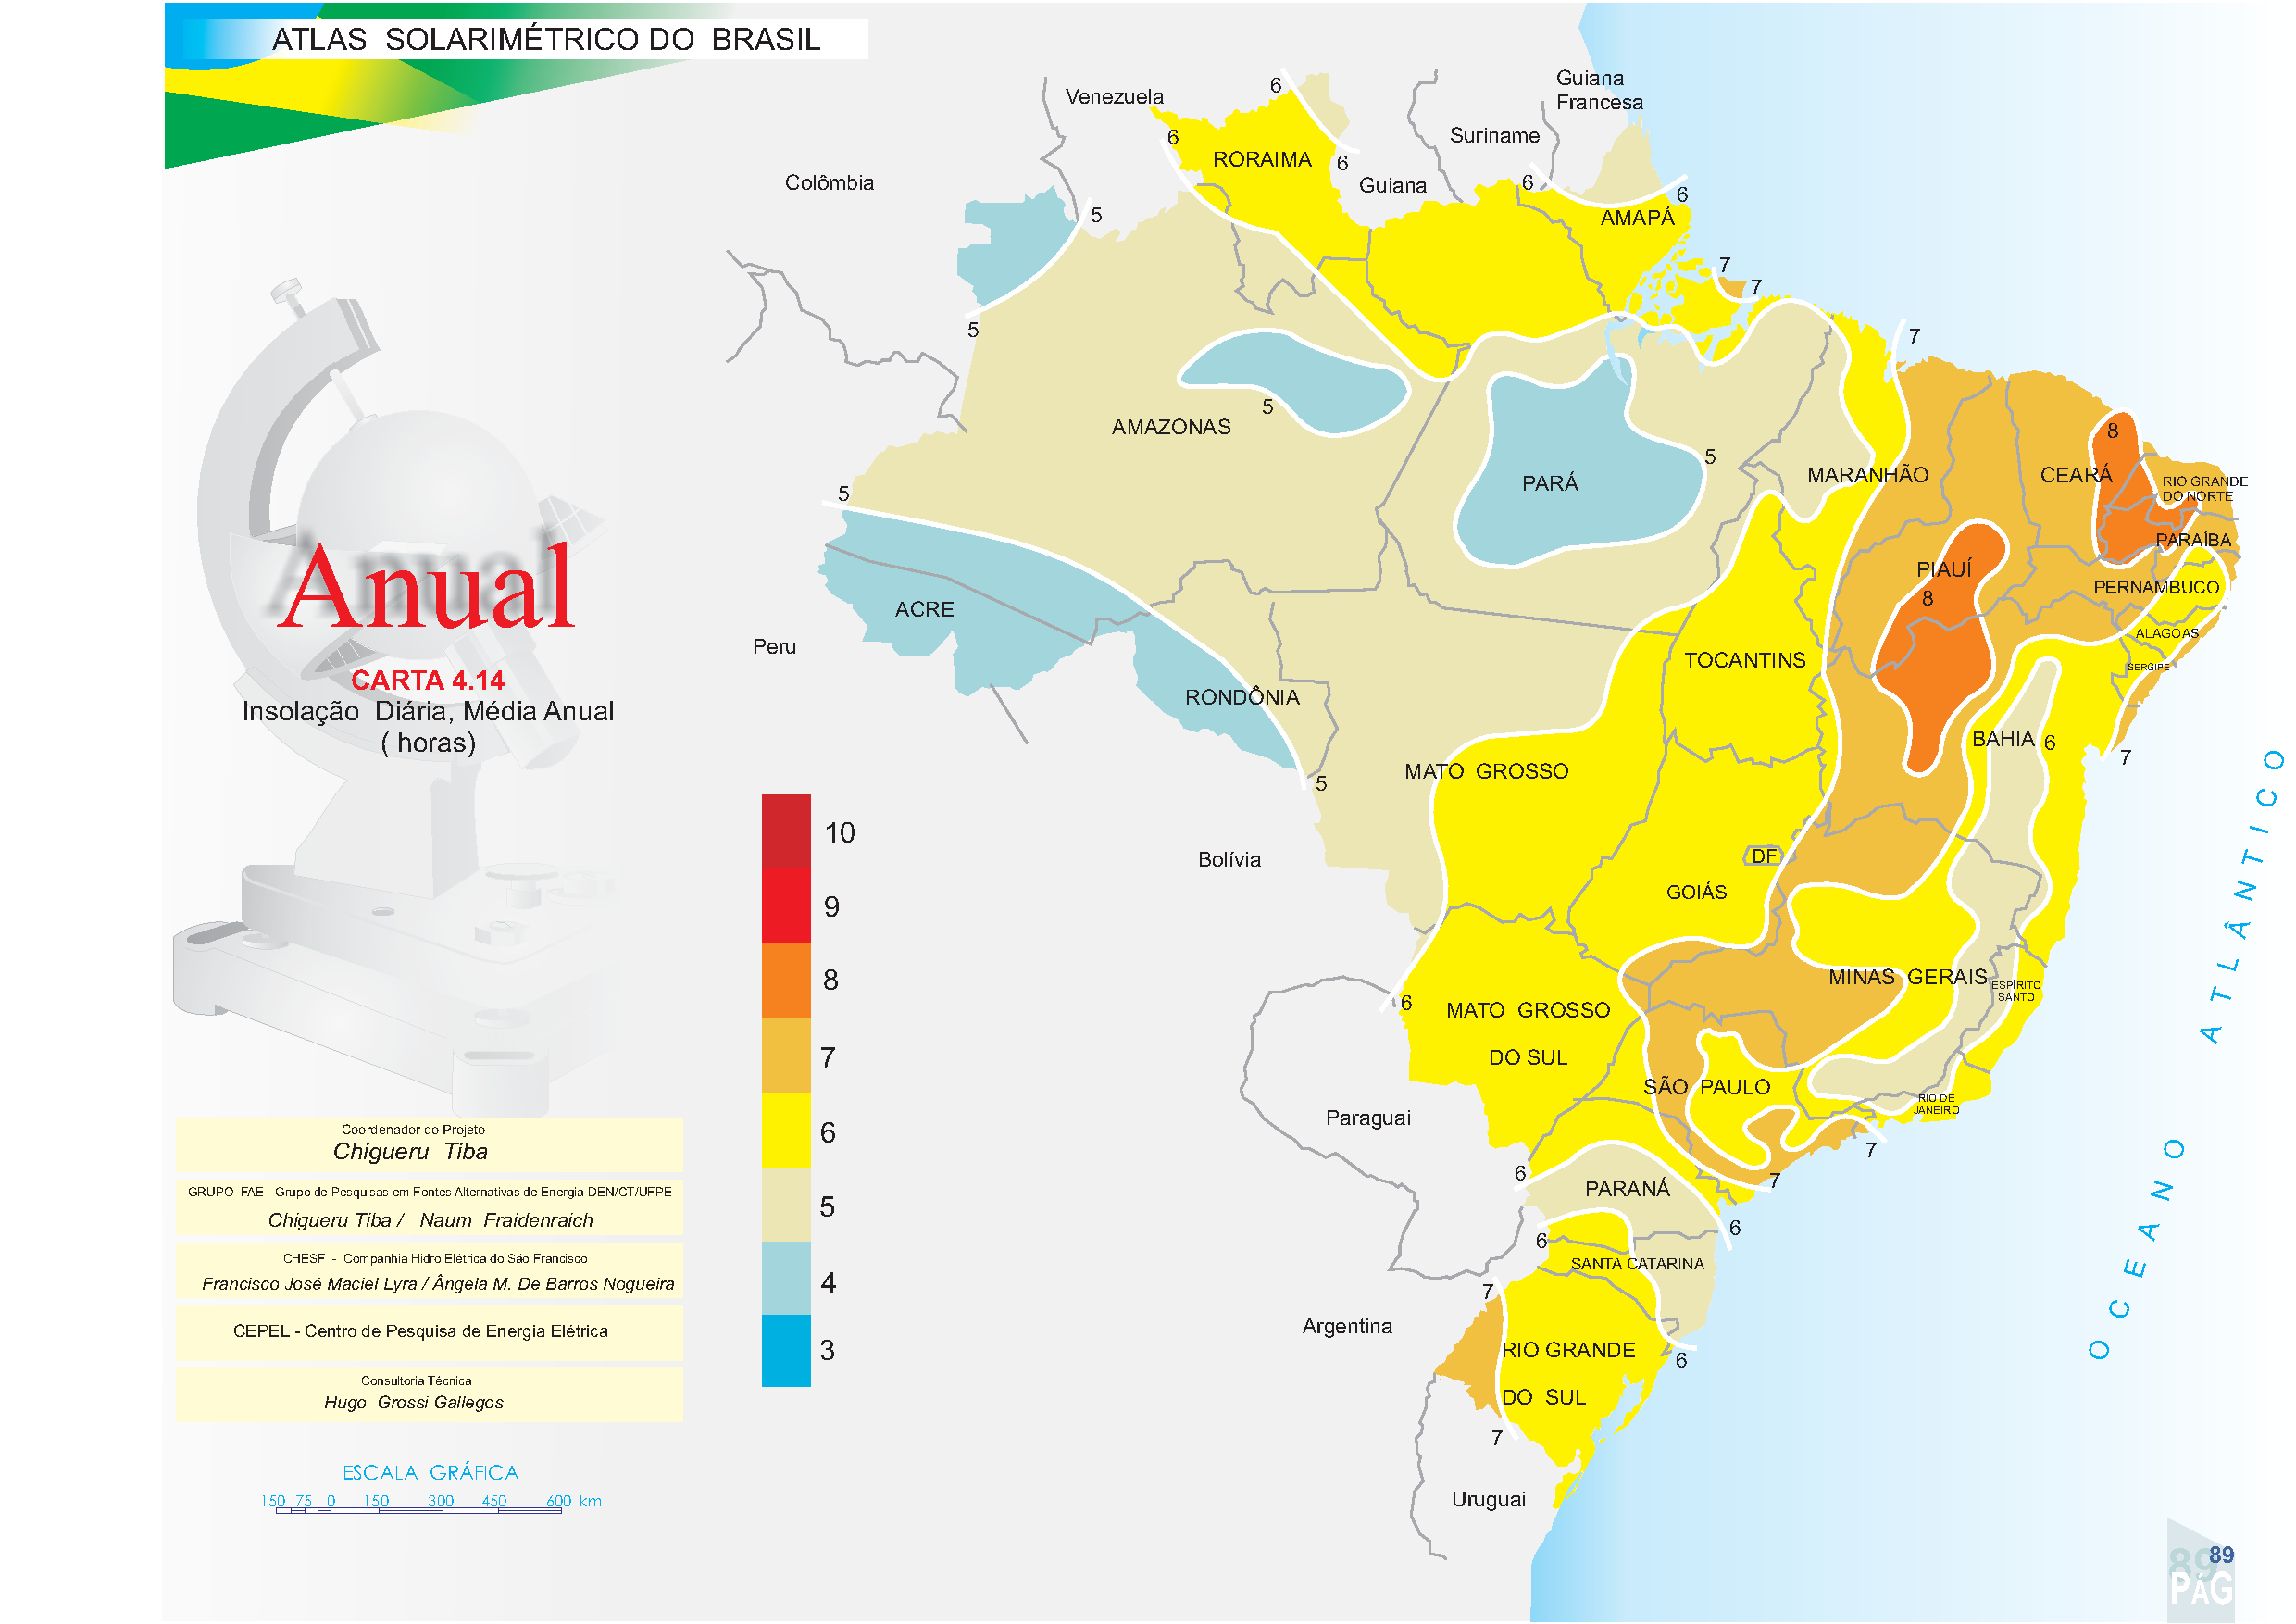
\includegraphics[scale=.25,center]{atlas_inso_ano}
\end{figure}

\end{frame}

\begin{frame}{Energia disponível no local}

São apresentadas duas metodologias de cálculo:

\vspace{.5cm}
		
\begin{columns}[T]
    \begin{column}{0.5\textwidth}
		\vspace{.5cm}
		\begin{itemize}
			\item Método da insolação
			\item Método da corrente máxima
		\end{itemize}
    \end{column}
    \begin{column}{0.5\textwidth}    
		\centering
      	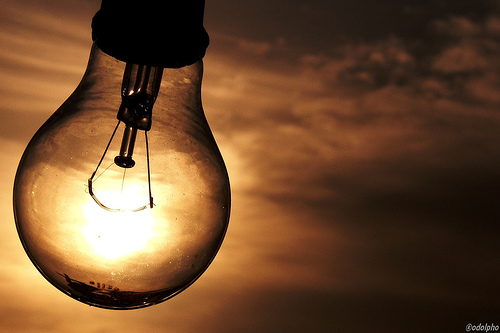
\includegraphics[scale=.25,center]{demanda}
    \end{column}
\end{columns}

\vspace{.5cm}
		
\begin{exampleblock}{}
\begin{center}
Objetivo: Atender a demanda de energia elétrica todos os dias do ano
\end{center} 
\end{exampleblock}

\end{frame}

\begin{frame}{Energia disponível no local}

\textbf{Método da insolação}

\vspace{.5cm}

\begin{footnotesize}
	\begin{equation*}
	\underset{Módulo}{Energia \, Produzida}\left [ \frac{kWh}{dia} \right ]=\underset{Diária}{Irradiação}\left [ \frac{kWh}{m^2 \cdot dia} \right ] \times \underset{Total \, Módulo}{Área }\left [ m^2 \right ] \times \underset{Módulo}{Eficiência}
	\end{equation*}
\end{footnotesize}

\vspace{.5cm}

\begin{exampleblock}{Considerações para a produção de energia}
	\begin{itemize}
		\item limitada pela eficiência do módulo
		\item varia sazonalmente (aumenta de acordo com a irradiação do pior mês do ano)
	\end{itemize}
\end{exampleblock}

\end{frame}

\begin{frame}{Energia disponível no local}

\textbf{Método da corrente máxima}

\vspace{.5cm}

\begin{footnotesize}
\begin{equation*}
\underset{Módulo}{Energia \, Produzida}\left [ \frac{kWh}{dia} \right ]=\underset{Módulo}{Potência}\left [ kW \right ] \times \underset{Total \, Horas}{Insolação}\left [ \frac{h}{dia} \right ]
\end{equation*}
\end{footnotesize}

\begin{footnotesize}
\begin{equation*}
\underset{Módulo}{Potência}\left [ kW \right ]=\underset{Curto-circuito}{Corrente}\left [ A \right ] \times \underset{Operaçñao}{Tensão}\left [ V \right ]
\end{equation*}
\end{footnotesize}

\begin{exampleblock}{Corrente de curto-circuito}
	\begin{itemize}
		\item STC - valores acima das condições de operação
		\item NOCT - valores mais próximos das condições de operação
	\end{itemize}
\end{exampleblock}

\end{frame}
